\documentclass[12pt,a4,notitlepage]{report}

\usepackage{verbatim,graphicx,fancyvrb,amsmath,url}

% \input{epsf}            % to allow postscript inclusions

\raggedbottom             % try to avoid widows and orphans
\sloppy
% \clubpenalty1000%
% \widowpenalty1000%

\setlength{\parindent}{0cm}
\setlength{\parskip}{2ex plus 1ex minus 0.5ex}
\addtolength{\evensidemargin}{-1.5cm}
\addtolength{\oddsidemargin}{-1.5cm}
\addtolength{\textwidth}{2.6cm}
\addtolength{\topmargin}{0.5cm}
\addtolength{\textheight}{2cm}
\addtolength{\footskip}{0.5cm}

\renewcommand{\textfraction}{0.15}
\renewcommand{\topfraction}{0.85}
\renewcommand{\bottomfraction}{0.65}
\renewcommand{\floatpagefraction}{0.60}

\renewcommand{\_}{\texttt{\symbol{95}}}
\newcommand{\<}{\texttt{\symbol{60}}}
\renewcommand{\>}{\texttt{\symbol{62}}}
\newcommand{\class}[1]{\textbf{#1}}
\newcommand{\scopendpoint}[1]{\texttt{#1}}
\newcommand{\variable}[1]{\texttt{#1}}
\newenvironment{pseudocode}{\begin{slshape}\begin{tabbing}\hspace*{0.5cm}\=\hspace*{0.5cm}\=\hspace*{0.5cm}\= \kill }{\end{tabbing}\end{slshape}}
\DefineVerbatimEnvironment{code}{Verbatim}{}
%\newcommand{\implies}{\Rightarrow}

\includeonly{propbody}

%\renewcommand{\baselinestretch}{1.1}    % adjust line spacing to make
%                                        % more readable

\begin{document}

\bibliographystyle{plain}

%%%%%%%%%%%%%%%%%%%%%%%%%%%%%%%%%%%%%%%%%%%%%%%%%%%%%%%%%%%%%%%%%%%%%%%%
% Title

\pagestyle{empty}

\hfill{\LARGE \bf Cheryl Hung}

\vspace*{30mm}
\begin{center}
\Huge
{\bf Gesture-controlled Robotics \\
using the Vicon Motion Capture System} \\
\vspace*{25mm}
Computer Science Tripos \\
\vspace*{5mm}
King's College \\
\vspace*{5mm}
\today  % today's date
\end{center}

\cleardoublepage

%%%%%%%%%%%%%%%%%%%%%%%%%%%%%%%%%%%%%%%%%%%%%%%%%%%%%%%%%%%%%%%%%%%%%%%%%%%%%%
% Proforma, table of contents and list of figures

\setcounter{page}{1}
\pagenumbering{roman}
\pagestyle{plain}

\chapter*{Proforma}

{\large
\begin{tabular}{ll}
Name:               & \bf Cheryl Hung                       \\
College:            & \bf King's College                     \\
Project Title:      & \bf Gesture-controlled Robotics using the \\
                    & \bf Vicon motion capture system \\
Examination:        & \bf Computer Science Tripos, 2009        \\
Word Count:         & \bf wordcount \\
Project Originator: & Cheryl Hung                    \\
Supervisor:         & Cecily Morrison, Laurel Riek                    \\ 
\end{tabular}
}

\section*{Original Aims of the Project}

This project aims to demonstrate the use of machine learning techniques for the purposes of gesture recognition. I have chosen to use full body motion capture as input, capturing three-dimensional kinematic data from arm gestures performed by users. The intention is to use two well known computational models, neural networks and hidden Markov models, in order to convert the gestures into commands to drive robots.

\section*{Work Completed}

\begin{itemize}
\item I have completed a module for real-time preprocessing of the raw input data, including translating relative arm coordinates into body coordinates.
\item In addition to the original two recognisers, I have implemented a further two recognisers, which are heuristics-based and aggregative respectively.
\item I recorded nearly a hundred gestures for use in training and evaluation, including multiple users and negative examples.
\item Finally, I have implemented the multiplayer extension, control for the physical robots and motion capture and also full simulations of both the coordinates stream and command stream.
\end{itemize}

\section*{Special Difficulties}

None
 
\newpage
\section*{Declaration}

I, Cheryl Hung of King's College, being a candidate for Part II of the Computer Science Tripos, hereby declare that this dissertation and the work described in it are my own work, unaided except as may be specified below, and that the dissertation does not contain material that has already been used to any substantial extent for a comparable purpose.

\bigskip
\leftline{Signed }

\medskip
\leftline{Date }

\cleardoublepage

\tableofcontents

\listoffigures

%%%%%%%%%%%%%%%%%%%%%%%%%%%%%%%%%%%%%%%%%%%%%%%%%%%%%%%%%%%%%%%%%%%%%%%
% now for the chapters

\cleardoublepage        % just to make sure before the page numbering
                        % is changed

\setcounter{page}{1}
\pagenumbering{arabic}
\pagestyle{headings}

\chapter{Introduction}

\section{Motivations}
New paradigms for human-computer interaction are becoming a reality. Amongst consumer goods, new ways of interaction encourage innovation beyond the keyboard and mouse. The Apple iPhone is the first touchscreen cellular phone to be widely adopted, while the Nintendo Wii brings accelerometer-based control to home gaming. The Opera browser uses mouse gestures for navigational input, while the Microsoft Surface is aimed towards diverse markets, from corporate events to restaurants.

The philosophy which is common to these systems is the convergence towards ``everyday" simplicity. The aim is to allow intuitive, natural interaction so that anybody (in theory) can use them without training, by mirroring or mimicking behaviour of the real world.

Robots, by contrast, have generally been operated by skilled engineers and researchers. The motivation was to bring the power of human intuition to the human-machine interface, using techniques from machine learning. The medium that I chose to investigate and exploit is gesture recognition, a specialization of pattern recognition.

\section{Project aims}

While machine vision is one option for obtaining user input, motion capture systems provide far more detailed location data, down to hundredths of a millimeter. Gesture recognition is a two-phase problem; the training with prerecorded datasets and the run-time interpretation. Rather than accepting arbitrary gestures as input, I chose to train on a finite set of predefined gestures, converting these into commands that are used to drive the robot. 

This project uses machine learning techniques for gesture recognition in order to control a remote vehicular robot. Three very different approaches were taken to the same problem; a heuristic evaluator, artifical neural networks, and hidden Markov models. The gesture data was recorded from a motion capture system using arm and body markers for training purposes and was preprocessed for invariance to translation and rotation before feature extraction. This allows users to be facing in any direction at any point, and also to move around the area whilst performing a gesture. A voting system was implemented to aggregate the results and intepret the real time data as commands. Furthermore, an extension for multiple users was implemented, and the system demonstrated successfully on live motion capture data to control physical hardware.

\chapter{Preparation}

\section{Requirements Analysis}

The project is divided into three phases; preprocessing of motion capture data, recognition and intepretation into commands, and execution on hardware. The overall requirement is that the system should allow the user to control a small robot using arm gestures, in real time. Broken down into subgoals:

\begin{itemize}
\item The system should implement multiple recognisers, including neural networks and hidden Markov models. In order to be transparent to the programmer, it should provide a consistent API for training and recognition for each classifier.
\item The system should receive data from the motion capture system and preprocess it in order to have the properties of location and rotation invariance.
\item The stream of raw data should be segmented into gestures without requiring an operator.
\item A training module should be read gesture data files from disk, train for a particular user, and save and load this trained state.
\item The system should be fully usable without any physical hardware; in other words, a simulation for a stream of coordinates and a representation of virtual robot.
\item Finally, the system should intepret the commands in order to drive the robot.
\end{itemize}

\subsection{Hardware}

The main requirements of the hardware were:

\begin{enumerate}
\item The system should accept a range of commands, in order to allow training of multiple gestures. A simple vehicle sufficed for this purpose.
\item The system should have wireless capabilities for independent movement.
\item The system should provide a high level API or library, for ease of development.
\item Purchasing multiple units for multiuser applications is easier with commercially available robots.
\item The system should have high battery life and low power consumption, for testing purposes.
\item The system should be relatively low cost (see budgeting for more)
\end{enumerate}

The main alternatives considered were:
\begin{enumerate}
\item Lego Mindstorms, already owned by the Computer Laboratory and including a C++ API, with purchased modules for wireless and touch sensors. This was dismissed as building a vehicle, testing for range of movement and so on would take excessive development time.
\item iRobot Roomba, a low cost vacuum cleaning robot with bump sensors, with third party peripherals for wireless and webcam. Reaching the serial ports on the Roomba would require removal of hardware and deconstruction of the vacuum innards.
\item iRobot Create\cite{Create}, an educational robot similar to the Roomba, without vacuum parts. A device for wireless could be attached by serial cable. A setup based on the OLPC Telepresence\cite{OLPCtelepresence} also provides a Python library for interfacing with both the laptop's webcam and robot's motors and bump sensors. \\
This was the option chosen, for ease of development and cost effectiveness.
\end{enumerate}

The budget was \pounds 500, funded equally by the Computer Laboratory Outreach programme and King's College. The final expenditure came to \pounds 585 as follows:

Two iRobot Creates at \$229.99 = \pounds 306.80 \\
OLPC XO laptop @ \$220.00 = \pounds 151.86 \\
OLPC XO laptop @ \$170.00 = \pounds 117.35 \\
UK/US Step Down Adapter = \pounds 8.99 \\
Total: \pounds 585.00

The main reason for the increase was that the basic iRobot Create comes without a rechargeable battery, and requires 12 AA batteries per robot per hour. The upgraded package comes with a command module as well as rechargeable battery; however it was found that the command module cannot be used, as it considers the laptop attached via USB to be a peripheral rather than the laptop being the USB master device to the robot slave.

\section{Motion Capture System}

The interface to the Vicon Motion Capture System in the Rainbow Group is provided by their proprietary software package Vicon Real-Engine, TARSUS\cite{Vicon}. This software collates the data from ten infra-red cameras to reconstruct the three dimensional marker positions in real time, and further combines these into either user-defined objects or full skeletons. There were two choices to be considered; the objects (body parts), and the gestures to be recognised.

The objects are needed firstly for input to a gesture, and secondly to represent the user's position so that the gestures can be calculated with invariance to translation and rotation. For the gesture input, one or two hands or arms were considered; two gives a wider range of movement (and thus a larger input space) and forearms have more rigidity than hands. This gives better recognition rates from the Vicon system because it increases the likelihood that the seen objects will match the saved body part.

Options for positional data were belt, hat and body. Having experimented with all three options, empirical results showed that the belt was easily occluded and confused by the arm markers, while the hat gave poor rotational data due to the independent movement of the head. The final configuration chosen was twelve markers spread across two arms and body (upper chest and back).

The data output is six data values per object; an Axis Angle triplet for rotation and a triplet for global translation in millimetres (mm). An alternative rotation system which is also available is Euler angles.

In order to simplify data processing while providing adequate control over the robot, most of the pre-set gestures were constrained to one arm movement within two dimensions (x-z or y-z planes in a z-up world). The commands chosen to provide basic steering and speed were accelerate, decelerate, turn left, turn right and start/stop, the latter being a test case for a more complex gesture, in this case a single clap at chest level. Figure \ref{gestures} shows the arm gestures for each command.

\begin{figure}
\centering
\includegraphics[scale=0.3,angle=0]{images/accel.ps}
\includegraphics[scale=0.3,angle=0]{images/decel.ps}
\includegraphics[scale=0.3,angle=0]{images/left.ps}
\includegraphics[scale=0.3,angle=0]{images/right.ps}
\includegraphics[scale=0.3,angle=0]{images/startstop.ps}
\caption{Top row: arm gestures for \textit{accelerate}, \textit{decelerate}, and \textit{turn right}. 
Bottom row: \textit{turn left}, and \textit{start/stop}.}
\label{gestures}
\end{figure}

\subsection{Axis Angles}

Axis angles are also known as exponential coordinates or rotation vectors. This parametrizes orientation by a three dimensional Cartesian vector, describing a directed axis and the magnitude of rotation. The rotation matrix shown in figure \ref{axisangle} is used to rotate around an arbitrary axis where $(x,y,z)$ is a unit vector on the axis of rotation, and $\theta$ is the angle of rotation.\cite{GraphicsGems}

\begin{figure}
$\theta = \sqrt{x^2 + y^2 + z^2}$\\

$c = \cos(\theta)$\\
$s = \sin(\theta)$\\
$t = 1-c $\\

$R =
\left( \begin{array}{ccc}
      tx^2+c & txy+sz & txz-sy\\
		txy-sz & ty^2+c & tyz+sx\\
		txz+sy & tyz-sx & tz^2+c\\
\end{array} \right)$
\caption{Axis angle rotation matrix.}
\label{axisangle}
\end{figure}

\subsection{Euler Angles}

With Euler angles, the rotation matrix is decomposed into three rotations from a reference frame, $(x,y,z)$. The rotated orientation system is denoted in upper case letters, $(X,Y,Z)$. The line of nodes (N) is the line of intersection between the $xy$ and $XY$ coordinate planes, and the new coordinate system is parametrised by $(\alpha,\beta,\gamma)$.

In the standard z-x-z convention,

\begin{itemize}
\item $\alpha$ is the angle between the x-axis and the line of nodes, modulo $2\pi$
\item $\beta$ is the angle between the z-axis and the Z-axis, modulo $\pi$
\item $\gamma$ is the angle between the line of nodes and the X-axis, modulo $2\pi$
\end{itemize}

\begin{figure}
\centering
\includegraphics[scale=0.2,angle=0]{diagrams/eulerangles.ps}
\caption{Euler Angles\cite{eulerangles}}
\label{eulerangles}
\end{figure}

However, when the $xy$ and $XY$ planes are identical and the $z$ and $Z$ axes are parallel, not all points in the coordinate system can be uniquely identified. This phenomenon known as {\em gimbal lock}. Euler angles are also prone to angle flips at the extremities of the ranges of $\alpha,\beta,\gamma$. For this reason, Euler angles are harder to deal with than axis angles, which vary smoothly.

\section{Pattern recognition}

There are many different techniques in the field of machine learning used for pattern recognition. The purpose of the pattern recognition phase is to classify the observations into categories, based on extracted features. For supervised learning, a training set of patterns is labelled with the correct classification; unsupervised learning (such as the K-means clustering algorithm) evaluate the raw, unlabelled data and attempt to infer the patterns, for example by minimizing the root mean squared error based on Euclidean distance. The implementation of hidden Markov models offer both learning techniques, in the form of the Baum-Welch algorithm and the K-means clustering algorithm. Backpropagation is the most standard supervised learning technique for neural networks.

Statistical techniques for pattern recognition are based on finding a classifier
$ h: X \mapsto Y $ which maps $x \in X$ to $y \in Y$ in a close approximation to the actual ground function $ g: X \mapsto Y $ where the training set $ (\mathbf x_1,y_1), ... , (\mathbf x_n, y_n) $ are instances of $X \times Y$ (the Cartesian product of the $X$ and $Y$ domains).

Among the more popular techniques are Support Vector Machines, naive Bayes classifier, k-nearest neighbour, neural networks and hidden Markov models. I chose the latter two as an example of a general classifier and temporal (or sequential) classifier respectively.

\subsection{Neural Networks}

An artificial neural network is an interconnected set of nodes which individually perform simple processing, but which exhibits complex behaviour as a whole system. This is the connectionist approach to pattern recognition from large sets of data, inspired by  biological neural networks. Each unit combines the inputs by means of an activation function, which {\em fires} or adjusts its output non-linearly based on the value of the input. Common choices for the activation function are the $\tanh = \frac{\sinh x}{\cosh x}$ function or the sigmoid function, which have the property of being differentiable:

\begin{figure}
\centering
\[ \phi(v_i) = 1/(1+e^{-v_i}) \]
\caption{The sigmoid function.}
\label{sigmoid}
\end{figure}

In the discussion I use the following notation:

$w_{ji}$ connects node $i$ to node $j$ \\
$a_{ij}$ is the activation for node, the weighted sum of the inputs = $\sum_i {w_{ji}z_i}$ \\
$g$ is the activation function \\
$z_j = g(a_j)$ \\
bias input = 1

The most common model is the multilayer perceptron\cite{NeuralPat}, where the overall structure is feedforward and there are three layers of nodes; an input layer, a hidden layer and an output layer.

\begin{figure}
\centering
\includegraphics[scale=0.6,angle=0]{diagrams/neural.ps}
\caption{Multilayer perceptron, with a single layer of hidden nodes. Each layer of nodes is fully connected with the next layer.}
\label{mlp}
\end{figure}

Since this is a supervised learning technique, the first phase is to present training data. The goal is to adjust the weights $w$ so as to minimise the overall error, denoted ${E}(\mathbf w)$. The training sequence is a vector of labelled inputs:

\[ s = ((\mathbf x_1,y_1), ... , (\mathbf x_m, y_m)) \]

The backpropagation algorithm is an application of gradient descent for minimization of error\cite{NeuralPat}. The first stage is to initialize w to a random set of weights. Calculate $E (\mathbf w)$; if this is greater than a threshold value, calculate the gradient $\partial E (\mathbf w) / \partial \mathbf w $ of $E(\mathbf w )$ at each point $w_i$ and adjust the weight vector to reduce the error:

\[
\mathbf w_{i+1} = \mathbf w_i - \alpha \left. \frac {\partial E(\mathbf w)} {\partial \mathbf w} \right| \mathbf w_i
\]

The forward propagation stage is to calculate $a_j$ and $z_j$ for all nodes, given an input example $p$.

\[
\frac {\partial E_p(\mathbf w)} {\partial w_{ji}} = \frac {\partial E_p(\mathbf w)} {\partial a_j} \frac {\partial a_j} {\partial w_{ji}} = \delta_j z_i
\]

where $\delta j = \frac {\partial E_p\mathbf w} {\partial a_j}$
and $ \frac {\partial a_j} {\partial w_{ji}} = \frac {\partial} {\partial w_{ij}} \left( \sum_k {z_kw_{jk}} \right) = z_i$

There are two cases for calculating $\partial_j$:

1. $j$ is an output node

\[
\delta j = \frac {\partial E_p (\mathbf w)} {\partial a_j} \\
 = \frac {\partial E_p (\mathbf w)} {\partial z_j} \frac {\partial z_j} {\partial a_j} \\
 = \frac {\partial E_p (\mathbf w)} {\partial z_j}  g'(a_j)
\]

2. $j$ is not an output node

\[
\delta j = \frac {\partial E_p (\mathbf w)} {\partial a_j}
 = \sum_{k \in \{k_1, k_2,\ldots,k_q\}} \frac {\partial E_p (\mathbf w)} {\partial a_k} \frac {\partial a_k} {\partial a_j}
 = g'(a_j) \sum_{k \in \{k_1, k_2,\ldots,k_q\}} {\delta_k w_{kj}}
\]

since $ \frac {\partial a_k} {\partial a_j} = \frac {\partial} {\partial a_j} \left( \sum_{k \in \{k_1, k_2,\ldots,k_q\}} { w_{ki} g(a_i) } \right) = w_{kj} g'(a_j) $

This gives the \textit{back-propagation formula}\cite{NeuralPat}:
\[
\delta j = g'(a_j) \sum_{k \in \{k_1, k_2,\ldots,k_q\}} {\delta_k w_{kj}}
\]

The importance of this result is the reduction in time complexity, as training neural networks is very time consuming. The majority of the work is done calculating $a_{ij} = \sum_i {w_{ji}z_i}$. Letting $W$ be the total number of weights and biases, there are $W$ derivatives to calculate for each weight. The naive approach of explicit evaluating each derivative numerically in $O(W)$ operations is therefore $O(W^2)$ in time complexity. By contrast,  backpropagation (using $\frac {\partial E_p(\mathbf w)} {\partial w_{ji}} = \delta_j z_i$ to calculate the derivatives) reduces the computational complexity to $O(W)$.

\subsection{Hidden Markov Models}

First order Markov processes are a class of statistical model in which the probability of being in some future state is only dependent on the current state. This is also known as the memoryless model, since the ``memory" or past states have no effect on the next state.\cite{AIModern}

\[ Pr(S_t|S_{0:t-1}) = Pr(S_t|S_{t-1}) \]

where $S_{0:t-1} = (S_0,S_1,...S_{t-1})$ is the set of states from time $0$ to time $t-1$.

\begin{figure}
\centering
\includegraphics[scale=0.6,angle=0]{diagrams/markov.ps}
\caption{Hidden Markov models}
\label{hmm}
\end{figure}

At each time $t$, a symbol is emitted from state $i$. For a Bakis HMM, the only options at $t+1$ are to stay in state $i$ or move to state $i+1$\cite{Bakis}. Each state is parametrized by an emission probability of staying in the same state and a transition probability of moving to state $i+1$.

A Hidden Markov Model is one where these probabilities characterizing the states are unknown, and for a training sequence, it is unknown which state the observation lies in. To find the probabilities, the Baum-Welch algorithm takes a vector of training sequences and iterates using Expectation-Maximization. The expectation is calculated by the forward-backward algorithm, which is an example of dynamic programming and the use of memoization to avoid recomputing solutions to sub-problems.

For a Markov Model, $Pr(E_t|S_t)$ is the sensor model and $Pr(S_t|S_{t-1})$ is the transition model. $Pr(S_0)$ denotes the prior state. The assumption is that the probabilities do not change over time, as the observations are stationary processes.

There are four basic inference tasks that can be calculated using this formalism\cite{AIModern}:

\begin{enumerate}
\item Filtering: deducing the current state that we might be in, $Pr(S_t|e_{1:t})$
\item Prediction: deducing the future state that we might be in, $Pr(S_t|e_{1:t})$ for some $T>0$
\item Smoothing: deducing the past state that we might have been in at time $T$, $Pr(S_t|e_{1:t})$ for some $0 \le t < T$
\item Viterbi path : deducing the most likely sequence of states so far, $\underset{s_{1:t}}{\operatornamewithlimits{argmax}}Pr(S_t|e_{1:t})$
\end{enumerate}

The Viterbi algorithm solves the final task, which finds the maximum of the probabilities of taking each path through the states:
\begin{eqnarray*}
\max_{s_{1:t}} Pr(s_{1:t},S_{t+1}|e_{1:t+1}) &=& c \max_{s_{1:t}} Pr(S_{t+1},s_t) Pr(e_{t+1}|S_{t+1}) Pr(s_{1:t}|e_{1:t}) \\
 &=& c Pr (e_{t+1}|S_{t+1}) \max_{s_t}\left( Pr(S_{t+1}|s_t) \max_{s_{1:t-1}} Pr(s_{1:t-1}|e_{1:t}) \right) \\
\end{eqnarray*}
The algorithm therefore walks forwards over all possible sequences, calculating the most likely sequence for reaching the final states and selecting the most likely sequence of states. The time complexity of the Viterbi algorithm is $O(t)$ in the length of the sequence, t, since it performs the forward message pass phase once per possible path. The space complexity is also linear in $t$, for storing the $t$ pointers which indicate the best stage sequence.\cite{AIModern}
\begin{pseudocode}
for each possible state sequence: \\
\>  for each state at time t, $s_t$: \\
\>\>    forward a message $m_{1:t}$ combining the filtered estimate $Pr(S_t|e_{1:t})$ and updated with \\\>\>the new observation, to give the probability of the best sequence reaching this state \\
\> return maximum of the probabilities and follow the pointers back to find the most likely\\
\>\> sequence
\end{pseudocode}
There are two major training algorithms, Baum-Welch and K-Means. Both of them are implementations of the Expectation-Maximization phase described above.

\subsubsection{Baum-Welch}

The Baum-Welch training algorithm was first introduced by Baum L.E. and Weiss, N\cite{Baum-Welch}. It is a two-phase algorithm; the first requires calculating the forward and backward probabilities to be passed as messages, and the second phase calculates the expected count of the particular transmission-emission pair.

\subsubsection{K-means}

The k-means algorithm, also known as Lloyd's algorithm\cite{K-Means}, is a heuristic solution to the NP-hard problem of partitioning data $x_1, x_2, \ldots, x_n$ into k-clusters, $S = s_1, s_2, \ldots, s_k (k < n)$ and minimizes the within-cluster sum of squares error:

\[
{\underset{S}{\operatornamewithlimits{argmin}}\sum_{i=1}^k \sum_{x_j \in S_i} {\|x_j-\mu_i\|}^2}
\]

where $\mu_i$ is the mean of $S_i$.

\section{Feature extraction}

Neural networks have a fixed number of input nodes and so variable length data must be converted to a fixed size feature vector. This technique, known as dimension reduction, also reduces the search space significantly, which reduces training times and can improve recognition rates.\cite{NeuralPat}

There are several ways of doing this. For a discretely sampled time series, as the position data, the Discrete Fourier Transform encodes the signal as a coefficients of linear combinations of basis functions in a new frequency domain.\cite{DFT} Haar wavelets are an alternative method which also uses linear combinations of wavelet functions, that can represent discontinuities better than the Fourier method.\cite{Haar}

However these techniques were deemed excessively complex for the purposes of gesture recognition which only has a finite set of planar gestures, as in my case. I have therefore assumed that the simpler method of extracting axis-aligned ranges of movement is sufficient for distinguishing the gestures without adding the computational overhead of these other techniques.

\section{Development environment}

The majority of the system was developed under Linux with the Ubuntu 8.10 distribution. Programming was using a mixture of NEdit, gedit, and the command line tools \texttt{javac}, \texttt{java} and \texttt{python}.

The XO laptops run a modified version of Fedora Linux, while the PC used during live capture runs Windows XP.

The SRCF (Student-Run Computing Facility\cite{SRCF}) is used as a central server for data transfer.

\subsection{Tools}

Subversion was used for version control, with Google Code Project Hosting providing backup support. The libraries used were:

\textbf{Joone}: Java Object Oriented Neural Engine \cite{Joone}\\
\textbf{Jahmm}: Java Hidden Markov Model \cite{Jahmm} \\
\textbf{SCOP}: Server COmmunication Protocol \cite{SCOP} \\
\textbf{PyRobot}: robotics control \cite{PyRobot}\\
\textbf{TARSUS}: motion capture

Rather than implementing all the algorithms from scratch as originally planned, I chose to use established libraries for my machine learning needs. This came about on advice from my supervisor and has reduced the workload in this case, to give me time to implement a more complete final system.

I researched several neural network libraries, including Joone\ref{Joone} and JavaNNS\ref{JavaNNS}. The Joone library has particularly good tools for writing third party modules, as well as support for distributed training, which would be useful for higher performance in the CPU intensive training stage.

Java libraries for Hidden Markov Models included Jahmm\cite{Jahmm}, jHMM, and HmmSDK. I chose Jahmm as it has a good API and support for processing of vectors.

Decoupling various components using SCOP allows message passing between different languages, which was 
important to allow the Java client to communicate with the Python robotics control. This also meant that I could use a bottom-up, modular approach to each sub-problem.

This dissertation was typeset using \LaTeX\, together with \texttt{bibtex}. The graphs shown in the evaluation were generated using \texttt{gnuplot}; other diagrams were created using Inkscape.

\subsection{Languages}

The choice of languages was based on ease of development, portability, availability of libraries, and type safety. Python was chosen for readability and rapid prototyping, while Java was used for interfacing with powerful libraries. In a few cases certain classes have been prototyped in Python before being ported to Java.

The robot control library, \class{PyRobot}, is written in Python. The client used to interface with the TARSUS system is written in Java\cite{bodyPaint}. Message passing of simple string data is handled by SCOP, which has ports to both Python and Java.

This project uses several architectures; the OLPC XO runs a modified version of Fedora Linux, the Tarsus system runs on Windows XP and the development environment was Ubuntu Linux. Therefore it is important to use architecture independent languages, making it easy to perform processing on a more powerful computer than the XO laptop.

\chapter{Implementation}

\section{System Overview}

\begin{figure}
\centering
\includegraphics[scale=0.6,angle=0]{diagrams/systemdiagram.ps}
\caption{System Diagram}
\label{sysdiag}
\end{figure}

Figure \ref{sysdiag} shows how components are decoupled for re-usability. During training, the training sequences are read from disk and preprocessed to form data for training the pattern recognition modules. When live, the data capture subsystem sends arrays of raw data values to the SCOP server. The preprocessing module additionally listens to the event stream for gesture data. The output from all three services is interpreted as one of five commands by Control and is sent to the SCOP server on a different stream. For testing purposes, a GUI provides alternative input methods of mouse and keystrokes.

The relay program on the XO laptop converts this into drive commands and the PyRobot library handles low level opcodes. The monitor shows the output for a turtle program which responds to the same commands, again for test purposes.

Message passing provides inter-language communication via an SCOP server running on the SRCF. Logically, the processing can take place on a remote computer, but for performance reasons, I chose to perform processing on the same machine that is used to collect Vicon data.

\subsection{Component Interfaces}

All SCOP messages are ASCII strings. Each class that interacts with the server has a name and can express an interest in one or more streams, or \scopendpoint{endpoints}, by opening sockets.

NB: All names in the following discussions containing \verb^p1^ have \verb^p2^ equivalents for the second player.

\subsection{Protocols and data formats}

This table shows the protocols for interaction between various components. The three major data streams indicated by \scopendpoint{coordserver}, \scopendpoint{ctrlserver} and \scopendpoint{statusserver} can be redirected completely independently in a way that is transparent to users. Modules publish events and subscribe to interests denoted \scopendpoint{p1*} under the SCOP identifiers \variable{*p1}. The \verb#^#, \verb#&# and \verb#|# refer respectively to whether an instance of a class can listen to a single endpoint (taking a command line argument for \scopendpoint{p1} or \scopendpoint{p2}), to both endpoints simultaneously, or to either one or two as needed. 

Figure \ref{dfd} shows how the system components are decoupled throughout. The robots are connected via 802.11 wireless.

There were two options for drive commands; accelerate and decelerate, or drive forwards and backwards for a set time. Accelerate and decelerate with continual motion was chosen to avoid users having to continually issue commands to their robot. Start/Stop was chosen to provide an instantaneous way to halt the robot. This meant that turning should also be a smooth turn, rather than {\em stop} followed by a {\em turn in place} and then a {\em start}. 

\begin{tabular}{l|p{2.5cm}p{4.5cm}p{4.5cm}}
\rule[-2mm]{0mm}{3mm}SCOP server & Endpoint & Event sources & Event sinks\\
\hline
\rule{0mm}{4.5mm}\variable{coordsserver} & \scopendpoint{p1coords} &
\scopendpoint{capturep1}, \scopendpoint{simulatep1} &
\scopendpoint{windowp1}\rule[-2mm]{0mm}{3mm}\\ \\

 & \multicolumn{3}{l}{\begin{minipage}{12.5cm}%
The \variable{coordsserver} transmits both players' streams of coordinates, labelled \scopendpoint{p1coords} and \scopendpoint{p2coords}. The data format consists of eighteen floating point values, followed by a string which expresses the case where possible failure of object tracking by TARSUS has caused a body part to drop out.
\texttt{\{}\\
\texttt{\hspace*{5mm}\<body-ax\>, \<body-ay\>, \<body-az\>, }\\
\texttt{\hspace*{5mm}\<body-tx\>, \<body-ty\>, \<body-tz\>,}\\
\texttt{\hspace*{5mm}\<leftarm-ax\>, \<leftarm-ay\>, \<leftarm-az\>,}\\
\texttt{\hspace*{5mm}\<leftarm-tx\>, \<leftarm-ty\>, \<leftarm-tz\>,}\\
\texttt{\hspace*{5mm}\<rightarm-ax\>, \<rightarm-ay\>, \<rightarm-az\>,}\\
\texttt{\hspace*{5mm}\<rightarm-tx\>, \<rightarm-ty\>, \<rightarm-tz\>,}\\
\texttt{\hspace*{5mm}\<"ok"|"dropout"\>}\\
\texttt{\}}\\

All double values are accurate to six significant figures, in decimal. The axis angles values (ax,ay,az) are denormalised and in degrees ($-180^{\circ}$ to $+180^{\circ} $). Lost objects (reported as (0,0,0) for the angles) are converted to (0,0,1) and the status field set to ``\variable{dropout}". When non-zero values appear the status field is reset to ``\variable{ok}". Translations (tx,ty,tz) are in millimetres. The default rate is 100fps.\rule[-2mm]{0mm}{3mm}
\end{minipage}}\\

\hline
\rule{0mm}{4.5mm}\variable{ctrlserver} & \scopendpoint{p1ctrl} &
\scopendpoint{controlp1}, \scopendpoint{windowp1} &
\scopendpoint{viewp1}, \scopendpoint{relayp1}\rule[-2mm]{0mm}{3mm}\\ \\

 & \multicolumn{3}{l}{\begin{minipage}{12.5cm}%
The \variable{ctrlserver} handles the output from gestures, as single lower case characters representing an accelerate, decelerate, turn left, turn right or start/stop command:

\texttt{\<"a"|"d"|"l"|"r"|"s"\>}

The commands may be acted upon by the simulated or physical robots. Typically, a user issued around one per second.\rule[-2mm]{0mm}{3mm}
\end{minipage}}\\

\hline
\rule{0mm}{4.5mm}\variable{statusserver} & \scopendpoint{p1status} &
\scopendpoint{windowp1} & \scopendpoint{feedbackp1}\rule[-2mm]{0mm}{3mm}\\ \\

 & \multicolumn{3}{l}{\begin{minipage}{12.5cm}%
This stream is a direct transcription of the \texttt{<"ok"/"dropout">} field of the coordinates. It reflects whether the data provided by TARSUS can be used for the purposes of recognition.

\texttt{\<"ok"|"dropout"\>}
\end{minipage}}\\
\end{tabular}

\begin{figure}
\centering
\includegraphics[scale=0.75,angle=0]{diagrams/dataflowdiagram.ps}
\caption{Data flow diagram}
\label{dfd}
\end{figure}

\subsection{Breakdown of components}

Class diagrams
{diagram: class diagram}

\section{Motion capture}

The Tarsus system triangulates markers using infra-red emitted from the cameras, which is bounced back from the reflective markers. It uses stereoscopic techniques to resolve these into world coordinates, using ten cameras for redundancy when a marker is occluded for whatever reason.

With three objects per user and six data-points per object, the Tarsus server sends eighteen or thirty six (for two players) values per frame via TCP/IP on port 800, at 100 frames per second.

\begin{tabular}{|c|} \hline 
\class{Capture} \\ \hline
\multicolumn{1}{|p{16cm}|}
{ \variable{int FRAME\_RATE \newline
public static void output(double[] data, int startpos, SCOP scop, String label) \newline
public static void main (String[] args)
} } \\ \hline
\end{tabular}

\begin{tabular}{|c|} \hline 
\class{DataParserR} \\ \hline
\multicolumn{1}{|p{16cm}|}
{ \variable{DataInputStream is \newline
DataOutputStream os \newline
String[] channels \newline
public double[] getData() \newline
private String[] parseInfoPacket() \newline
private void matchStrings(String[] channels) \newline
private double[] parseDataPacket() throws IOException \newline
private static int readNum(DataInputStream is) throws IOException \newline
private static double readDoub(DataInputStream is) throws IOException
} } \\ \hline
\end{tabular}

The \class{Capture} class uses the Java client \class{DataParserR.java} to multiplex on the requested channel names, determining whether one or two players are currently using the system. It opens up to two sockets to a SCOP server running on localhost and forwards \scopendpoint{p1coords} and \scopendpoint{p2coords} to the gesture recognition phase. It also performs downsampling to a configurable frame rate (default is 100fps) to reduce burstiness and to avoid overloading the server buffers.

There are two potential problems with the data: glitches and dropouts. 
\begin{itemize}
\item Glitches are caused by incorrect object reconstruction. They are transcribed as valid data values from an object which have a high rate of change in a brief period. For example, a glitch could be: \\
\texttt{-1, -2, -1, 53, 168, 168, 89, -4, -3, 0, \ldots}

\item Dropouts are the result of improper triangulation from the cameras, and so the objects are not recognised at all and result in all rotational data being reported as 0.0 and translation data repeated from the last known values. A dropout is reported as: \\
\texttt{33, 33, 34, 35, 35, 0, 0, 0, 0, 36, 35, 35, \ldots} (rotation) \\
\texttt{697, 692, 680, 669, 669, 669, 669, 669, 669, 624, \ldots} (translation)
\end{itemize}

Dropouts are handled gracefully by setting a 19th flag in the stream, and converting rotations smaller than a given $\epsilon$ into harmless zero rotations about the Z-axis during preprocessing. Glitches are relatively hard to detect, relatively harmless, and the solution for fixing is less clear, so they are currently ignored.

\subsection{Training data}

Training data consists of five sequences for each of the five gestures, giving a total of twenty five gestures taken from each session, recorded by two users for robustness. The total number of input vectors used for training was 75.

In addition, two extra sets were recorded. The first is for calibration, consisting of stationary data at the origin, axis aligned translations, and 90 degree rotations. The second is examples of non-gestures, such as the neutral arms by side position. These provided negative examples to the pattern recognition engine.

The data is formatted as comma-separated values (CSV) files, as in figure \ref{trainingfile}. All values are double precision floating point numbers to six significant figures. Rotations are in the range $ \pm 180^{\circ}$ and translations are in millimetres from the origin in a z-up world.

\begin{figure}
\centering
{\scriptsize
\begin{verbatim}
BodyP1
Frame,BodyP1<A-X>,BodyP1<A-Y>,BodyP1<A-Z>,BodyP1<T-X>,BodyP1<T-Y>,BodyP1<T-Z>,
1,-0.991818,3.4194,-102.972,-715.545,820.366,1186.36,
2,-0.987695,3.40335,-102.978,-715.479,820.352,1186.33,
...
242,-1.61596,3.84801,-101.36,-696.667,821.255,1186.13,

LeftArmP1
Frame,LeftArmP1<A-X>,LeftArmP1<A-Y>,LeftArmP1<A-Z>,LeftArmP1<T-X>,LeftArmP1<T-Y>,LeftArmP1<T-Z>,
1,106.316,100.107,-19.2348,-660.681,1039.83,928.706,
2,106.457,99.9967,-19.219,-660.629,1039.9,928.689,
...
242,106.069,102.104,-19.6354,-649.414,1042.67,927.508,

RightArmP1
Frame,RightArmP1<A-X>,RightArmP1<A-Y>,RightArmP1<A-Z>,RightArmP1<T-X>,RightArmP1<T-Y>,RightArmP1<T-Z>,
1,27.848,44.5584,-47.155,-670.526,559.707,938.067,
2,28.3683,44.5345,-47.6479,-670.71,559.914,937.873,
...
242,30.3788,43.5149,-55.0284,-642.649,555,938.528,
\end{verbatim}
}
\caption{An example of a typical training file.}
\label{trainingfile}
\end{figure}

The following two classes are used for training purposes. \class{GestureReader} reads in and parses the data from disk, while \class{SimGesture} simulates a live user performing those gestures. This allows the recognition engine to be tested without needing a live data stream from the Vicon system.

\begin{tabular}{|c|} \hline 
\class{GestureReader} \\ \hline
\multicolumn{1}{|p{16cm}|}
{ \variable{public static ArrayList\<Frame\> getData(String filename) \newline
static SixDOF parse(String s)
} } \\ \hline
\end{tabular}

\begin{tabular}{|c|} \hline 
\class{SimGesture} \\ \hline
\multicolumn{1}{|p{16cm}|}
{ \variable{static ArrayList\<RecordedGesture\> read\_gesture(String gesture\_dir) \newline
public static void interpolate\_gestures(SCOP scop, RecordedGesture from\_gesture, RecordedGesture to\_gesture, int duration) \newline
private static Frame interpolate\_frames(Frame from, Frame to, double weight) \newline
private static SixDOF interpolate\_sixdof(SixDOF from, SixDOF to, double w) \newline
public static double interpolate\_angle(double from, double to, double w) \newline
static void framesync() \newline
public static void replay\_gesture(SCOP scop, RecordedGesture gesture)
} } \\ \hline
\end{tabular}

The \class{GestureReader} class contains a \variable{getData()} method, which reads in the data line by line until it finds an object name it recognises (``BodyP1", ``LeftArmP2" etc), ignores the column headings, and parses each frame until it finds whitespace. Each frame becomes a \class{Frame} object, containing references to three \class{SixDOF} objects for body, left arm and right arm. The \class{SixDOF} (six degrees of freedom) holds the six double precision floating point numbers corresponding to \<R-X\>, \<R-Y\>, \<R-Z\>, \<T-X\>, \<T-Y\>, \<T-Z\>; calling \variable{normalise()} sets the angle of rotation and normalises the rotation tuple to a unit vector. \\
The \class{SimGesture} class is used to replay the data in the same format as a Vicon stream on the same SCOP stream, rendering it identical to the real data. It uses \class{GestureReader.getData(filename)} on all CSV files from a single person and replays them in a random order. It assumes that all recorded gestures begin and end in the neutral position, and so movement between gestures is represented by linearly interpolating all values for a random length of time. It also appends the dropout boolean, in the same way as \class{Capture}.

\subsection{Preprocessing}

The data requires significant preprocessing to convert the feature vector from world coordinates to body coordinates. This is performed by the \class{Transform} class together with the \class{SixDOF}, \class{Frame}, and \class{Point} classes.

\begin{tabular}{|c|} \hline 
\class{Transform} \\ \hline
\multicolumn{1}{|p{12cm}|}
{ \variable{static void process(ArrayList<Frame> data) \newline
static void process(Frame f)
} } \\ \hline
\end{tabular}

\begin{tabular}{|c|} \hline 
\class{SixDOF} \\ \hline
\multicolumn{1}{|p{8cm}|}
{\variable{double ax, ay, az, angle, ty, ty, tz \newline
  static final double EPSILON = 1.0e-5 \newline
  SixDOF(double[] a, int offset) \newline
  public void normalise() \newline
  public String toString() \newline
  void rotate (double bearing) \newline
  double calcHeading() \newline
  void translate(SixDOF axes)
} } \\ \hline
\end{tabular}

The \class{SixDOF} class holds doubles for \variable{ax,ay,az,tx,ty,tz} and converts the \variable{ax,ay,az} Axis Angle triplet into a normalised vector plus an angle for the rotation magnitude. It converts small rotations into a zero rotation about the z-axis in order to avoid floating point errors.

\begin{tabular}{|c|} \hline 
\class{Frame} \\ \hline
\multicolumn{1}{|p{8cm}|}
{\variable{SixDOF body, left, right \newline
  Frame(String s) \newline
  Frame(double[] a, int offset) \newline
  public String toString() \newline
  public double[] toDoubles()
} } \\ \hline
\end{tabular}

The \class{Frame} class contains three of these \class{SixDOFs} for body, left arm and right arm. It has multiple constructors for loading from file or live stream, and can also be converted back to the same formats.

\begin{tabular}{|c|} \hline 
\class{Point} \\ \hline
\multicolumn{1}{|p{16cm}|}
{\variable{static final double EPSILON = 1.0e-5 \newline
  Point(double x, double y, double z)\newline
  static Point rotatePoint(double ax, double ay, double az, double angle, double x0, double y0, double z0)
} } \\ \hline
\end{tabular}

\class{Point} contains a static \variable{rotatePoint} method which implements the conversion from axis-angle triplets to matrix rotations. It takes an axis angle and a point to be rotated and returns a \class{Point}.

\begin{code}
double ax, ay, az, angle; //axis angle
double x0, xy, xz; //Point

double s = Math.sin(-angle);
double c = Math.cos(-angle);
double t = 1 - c;

Point p = new Point();

p.x = (t*ax*ax + c)*x0 + (t*ax*ay + s*az)*y0 + (t*ax*az - s*ay)*z0;
p.y = (t*ax*ay - s*az)*x0 + (t*ay*ay + c)*y0 + (t*ay*az + s*ax)*z0;
p.z = (t*ax*az + s*ay)*x0 + (t*ay*az - s*ax)*y0 + (t*az*az + c)*z0;
\end{code}

\subsection{Gesture segmentation}

The raw gesture data consists of a stream of vectors of 18 double-precision floating-point numbers, at 100 frames per second. In order to discover the start and end of gestures, the recogniser is repeatedly run on multiple rectangular windows of different sizes until a success is reported. Since the preprocessing and feature extraction is performed on every frame, I have implemented an optimization using dynamic programming to store processed frames in a circular buffer containing the last 500 frames of data.

\begin{tabular}{|c|} \hline 
\class{SlidingWindow} \\ \hline
\multicolumn{1}{|p{16cm}|}
{ \variable{static User user \newline
static Person person \newline
static Classifier classifier \newline
static SCOP scopin, scopout, scopstat \newline
static String player \newline
private static boolean recognised(CircularBuffer buf, int windowsize,	int framecounter)
} } \\ \hline
\end{tabular}

\begin{figure}
\centering
\includegraphics[scale=0.5,angle=0]{diagrams/slidingwindow.ps}
\caption{Accessing beyond the length of the circular buffer causes the index to wrap around to overwrite the beginning.}
\label{circbuf}
\end{figure}

\begin{tabular}{|c|} \hline 
\class{CircularBuffer} \\ \hline
\multicolumn{1}{|p{16cm}|}
{ \variable{CircularBuffer(int size, Frame init) \newline
private Frame[] circ \newline
private int ptr, size \newline
void add(Frame f) \newline
Frame get(int windowsize, int index)
} } \\ \hline
\end{tabular}

A circular buffer holds a list of frames and a pointer to indicate the next position for an incoming data frame. \class{SlidingWindow} performs preprocessing on  incoming frames, adds them to the active position until the buffer is full, and from then on overwrites the oldest frames.

Every ten frames, SlidingWindow runs the specified recogniser on the circular buffer with a range of window sizes from 50 frames (0.5 seconds) to 350 frames (3.5 seconds). Trials show that almost all clearly defined gestures fall within these boundaries.

\begin{pseudocode}
Loop forever: \\
\>	Get message from SCOP \\
\>	Add received frame to circular buffer \\
\>\>    for windowsize = 50 to 350, step size = 10 \\
\>\>        if (command recognised in circular buffer window) \\
\>\>\>           emit the command to ctrlserver
\end{pseudocode}

If a gesture is recognised from the current window, the buffer continues to fill with arriving data but no more attempts at recognition are made until the minimum windowsize is exceeded. In addition, \class{SlidingWindow} monitors the frames for a flag indicating a dropout; if a frame contains data where at least one object is unavailable, it emits a ``dropout" message to the \variable{statusserver}, and ``ok" when the object returns.

This status information is used by \class{Feedback.py} to display two rectangles, for player 1 and player 2, as in figure \ref{feedback}. A red rectangle indicates that the data is currently unavailable, while a green rectangle indicates a good detection rate. This feedback was highly rated in my user study of the system, allowing users to distinguish between poor detection from the Vicon system and poor recognition from a recogniser.

\begin{figure}
\centering
\includegraphics[scale=0.4,angle=0]{images/feedback.ps}
\caption{Feedback listening to \scopendpoint{p1status} and \scopendpoint{p2status} and showing that \scopendpoint{p1status} has reported a dropout.}
\label{feedback}
\end{figure}

\subsection{Feature extraction}

Neural networks have a fixed number of input nodes, but the feature vector has a variable number of frames. Therefore it is also necessary to perform feature extraction to create a fixed size set of variables to characterise the gesture. Performing feature extraction also reduces the search space for the recogniser, in order to increase the probability of successful matching. The gesture contains a lot of redundancy, since frames are taken at a high frame rate and show close temporal correlation.

Choosing the minimal features which extracted the most information to distinguish the gestures was an important step. Using the entire data for each gesture (6 data points * 3 objects * ~300 frames/gesture = 5400 data values, for each example) would be equivalent to template matching and would require excessive processing times. Since the gestures were chosen to be axis aligned relative to the body, the distinguishing features are the range of dx,dy,dz values that each prototypical gesture may take, which is not sensitive to factors such as the person's height or their neutral posture.

Each gesture is symmetric and begins and ends with a neutral pose, so I defined a further ``relocation" feature indicating a closed gesture: a double defining the sum of squares error of the distance moved from the beginning. Thus a gesture which is at the peak displacement will have a large relocation value, while a closed gesture which has returned to the starting pose has a small displacement value.

The seven features which are extracted are LeftArm {\em\{dx,dy,dz\}} and RightArm {\em\{dx,dy,dz\}}, normalised to between 0 and 1, and {\em displacement}, the sum of squares error of the first and last frames, in millimetres.

\begin{tabular}{|c|} \hline 
\class{Features} \\ \hline
\multicolumn{1}{|p{12cm}|}
{\variable{Features(ArrayList\<Frame\> data) \newline
Features(CircularBuffer buf, int windowsize) \newline
Ranges leftarm, rightarm \newline
double displacement \newline
double calc\_displacement(Frame first, Frame last) \newline
void extract(double[] a)
} } \\ \hline
\end{tabular}

Ranges is a utility class which contains six values for the minimum and maximum of x, y and z.  It takes a list of Frames and holds two Ranges for left and right arms, and a double containing the displacement value calculated as follows:
\begin{code}
double displacement = 0.0;
displacement += square(last.left.tx - first.left.tx);
displacement += square(last.left.ty - first.left.ty);
displacement += square(last.left.tz - first.left.tz);
displacement += square(last.right.ax - first.right.ax);
displacement += square(last.right.ay - first.right.ay);
displacement += square(last.right.az - first.right.az);
\end{code}
\section{Recognition}

\subsection{Recogniser}

The \class{Recogniser} is a base class which defines an interface containing two method that all recognisers are expected to override, namely \variable{train} and \variable{recognise}.

\begin{tabular}{|c|} \hline 
\class{Recogniser} \\ \hline
\multicolumn{1}{|p{16cm}|}
{\variable{public static Gesture recognise(Person person, Features features) \newline
public void train(ArrayList<Sample> samples, String out\_file)
 } } \\
\hline
\end{tabular}

\class{Gesture}, \class{Person} and \class{Classifier} classes are type-safe enumerations of the valid inputs. They provide accessor and mutator methods, and can be transformed into commands, strings, persons and so on.

\begin{tabular}{|c|} \hline 
\class{Gesture} \\ \hline
\multicolumn{1}{|p{8cm}|}
{\variable{TurnLeft \newline TurnRight \newline Accelerate \newline Decelerate \newline StartStop \newline NoMatch \newline MultiMatch \newline
Gesture(int cmd) \newline
public String toAction() \newline
public String toString() \newline
static Gesture lookup(String name) \newline
public boolean equals(Gesture g)
} } \\ \hline
\end{tabular}

\begin{tabular}{|c|} \hline 
\class{User} \\ \hline
\multicolumn{1}{|p{8cm}|}
{\variable{CHERYL \newline DAVID \newline
User(int who) \newline
private int userid \newline
String name() \newline
void set(int who) \newline
Person get\_person() \newline
static String all\_usernames() \newline
static int lookup(String name)
} } \\ \hline
\end{tabular}

\begin{tabular}{|c|} \hline 
\class{Classifier} \\ \hline
\multicolumn{1}{|p{12cm}|}
{\variable{HEURISTIC \newline NEURAL \newline MARKOV \newline HYBRID \newline
Classifier(int which) \newline
private int id \newline
String name() \newline
void set(int which) \newline
static String all\_classifiers() \newline
static int lookup(String name) \newline
Gesture recognise(Person person, Features features) \newline
void train(ArrayList<Sample> samples, String out\_file)
} } \\ \hline
\end{tabular}

The \class{Person} class is the union of all trained data related to a single specified user. It aggregates \class{Interval}s, neural network and hidden Markov model parameters, and also contains a constructor populating these fields from data files.

\begin{tabular}{|c|} \hline 
\class{Person} \\ \hline
\multicolumn{1}{|p{8cm}|}
{\variable{Intervals[] left, right \newline String neural\_file \newline NeuralNet nnet \newline DirectSynapse netout \newline int neural\_seq  \newline String markov\_root \newline Person()
} } \\ \hline
\end{tabular}

\subsection{Heuristic recogniser}

\begin{tabular}{|c|} \hline 
\class{Heuristic extends Recogniser} \\ \hline
\multicolumn{1}{|p{16cm}|}
{\variable{static double CLOSED\_THRESHOLD \newline
public static Gesture recognise(Person person, Features features) \newline
private static boolean match(Person person, Features features, int gesture)
} } \\ \hline
\end{tabular}

\begin{tabular}{|c|} \hline 
\class{Intervals} \\ \hline
\multicolumn{1}{|p{12cm}|}
{\variable{private double[][] range \newline
  double get\_min(int axis) \newline
  double get\_max(int axis) \newline
  void setX(double from, double to) \newline
  void setY(double from, double to) \newline
  void setZ(double from, double to) \newline
  void stationary(int wobble)
} } \\ \hline
\end{tabular}

This application-specific recogniser depends strongly on the particular gestures chosen. It makes use of prior knowledge about the domain; specifically, patterns for how each gesture is characterised.

The first off-line training stage is to calculate all features on the training dataset, excluding outliers. The \class{Person} class defines the valid intervals of the specified user for the left and right ranges, as the maximum and minimum ranges that are permissible. The threshold for a closed gesture was experimentally determined to be around 3000$mm^2$, but is editable in the configuration file.

When given a \class{Person} and \class{Features} calculated from a list of frames, the first check is that the displacement is less than the specified threshold. If this succeeds, the left and right \class{Range}s are compared with the \class{Person}'s \class{Interval}s. If the ranges fall within the permissible intervals, a \class{Gesture} is returned.

\subsection{Neural network recogniser}

\begin{tabular}{|c|} \hline 
\class{Neural extends Recogniser implements NeuralNetListener} \\ \hline
\multicolumn{1}{|p{16cm}|}
{ \variable{+ static Gesture recognise(Person person, Features features) \newline
+ void train(ArrayList<Sample> sampleslist, String out\_file) \newline
- void init\_parameters() \newline
static void saveNeuralNet(NeuralNet nnet, String filename) \newline
static NeuralNet restoreNeuralNet(String filename) \newline
void set\_columns(MemoryInputSynapse syn, int first, int last) \newline
+ void errorChanged(NeuralNetEvent e) \newline
+ void netStarted(NeuralNetEvent e) \newline
+ void netStopped(NeuralNetEvent e) \newline
+ void netStoppedError(NeuralNetEvent e, String error) \newline
+ void cicleTerminated(NeuralNetEvent e)
} } \\ \hline
\end{tabular}

There are seven input nodes corresponding to the seven features, a variable number of nodes in the hidden layer and five output nodes indicating a single gesture. Each gesture is labelled with a vector of expected output; for example, an accelerate gesture is \variable{(1,0,0,0,0)}, a Turn Right gesture is \variable{(0,0,0,1,0)} and a non-gesture is \variable{(0,0,0,0,0)}.

The output of this is the list of weights which can be saved to disk. The Joone library is structured using the callbacks \variable{errorChanged}, \variable{netStarted}, \variable{netStopped}, \variable{netStoppedError} and \variable{cicleTerminated} [sic], which are defined in the \class{NeuralNetListener} interface.

Training can be done in one of three modes; the standard Backpropagation algorithm, batch mode, and Resilient Backpropagation, an alternative which only uses the sign of the gradient rather than the magnitude and thus generally converges much faster.

\subsection{Hidden Markov Model recogniser}

\begin{tabular}{|c|} \hline 
\class{Markov extends Recogniser} \\ \hline
\multicolumn{1}{|p{16cm}|}
{ \variable{+ static Gesture recognise(Person person, Features features) \newline
+ void train(ArrayList<Sample> samples, String out\_file) \newline
- static ArrayList<ObservationVector> toObservationVectors(ArrayList<Frame> frames) \newline
static void save\_hmm(Learner learner, String filename) \newline
static Hmm restore\_hmm(String filename) \newline
- void init\_parameters()
} } \\ \hline
\end{tabular}

\begin{tabular}{|c|} \hline 
\class{Learner} \\ \hline
\multicolumn{1}{|p{16cm}|}
{ \variable{Learner(int states, int dimensions, int iterations, Gesture g) \newline
void add\_sequence(ArrayList<ObservationVector> seq) \newline
void learnbw() \newline
void learnkm()
} } \\ \hline
\end{tabular}

Each gesture is modelled by a different Markov process, so five hidden Markov models are created for the five gestures. This recogniser uses the raw data rather than the extracted data, since it is highly dependent on the temporal characteristics of the input vector.

Two learning algorithms are used, Baum-Welch (\variable{learnbw()}) and K-Means clustering (\variable{learnbw()}). The Baum-Welch iteratively improves on a starting hidden Markov model, and so one iteration of k-means is used to initialise the Baum-Welch training. Since the training sequences used are relatively long, a modification known as the Baum-Welch Scaled Learner is used, and the results reported as natural logarithms of probabilities to avoid underflow.

The recognition phase is an implementation of the Viterbi algorithm which finds the most likely state sequence, which corresponds to the most likely gesture issued by the user.

\newpage

\subsection{Decision logic}

\begin{tabular}{|c|} \hline 
\class{Hybrid extends Recogniser} \\ \hline
\multicolumn{1}{|p{16cm}|}
{ \variable{+ static Gesture recognise(Person person, Features features) \newline
+ void train(ArrayList<Sample> samples, String out\_file)
} } \\ \hline
\end{tabular}

This aggregates the results from each recogniser and uses a majority voting system to decide which, if any, are correct. The output of each recogniser is a single gesture, so any two recognisers matching is considered correct. The training method calls the \variable{train} on the neural network and hidden Markov model recognisers, as training is not valid for the heuristic recogniser.

This is an application of the safety engineering technique of triple modular redundancy. If any one of the methods fails to recognise the gesture or comes to an incorrect decision, the voting logic can use the other two pattern recognition techniques to mask the failure.

\subsection{Training}

\begin{tabular}{|c|} \hline 
\class{Training} \\ \hline
\multicolumn{1}{|p{12cm}|}
{\variable{User user \newline
Classifier classifier \newline
Training(ArrayList<Sample> samples, Classifier clf)
} } \\ \hline
\end{tabular}

\begin{tabular}{|c|} \hline 
\class{Sample} \\ \hline
\multicolumn{1}{|p{12cm}|}
{\variable{String pathname \newline
Gesture gesture \newline
ArrayList\<Frame\> \newline
Features feat \newline
Sample(String pathname, Gesture g)
} } \\ \hline
\end{tabular}

The offline training phase is implemented with a Training class and a set of Samples. The constructor calls the \variable{train()} method on the specified classifier, and can be used as a command line tool on a directory of gestures. This can be used to train a classifier and save the results to a data file.

\section{Framework}

\subsection{Simulated control}

Two graphical user interfaces were created which simulated input (via mouse and keyboard) and output (turtle graphics) respectively for alternative feedback. These were completely decoupled and communicated only via the SRCF. Since these were independent from the rest of the system, they are written in Python using the Python SCOP library and Tkinter, the Python graphical libraries. I used the Model-View-Controller design pattern to separate display from control:

\begin{itemize}
\item \class{control} displays a control panel which accepts either keystrokes or mouse clicks and emits commands on either the \scopendpoint{p1ctrl} or the \scopendpoint{p2ctrl} streams.

\begin{figure}[hb]
\centering
\includegraphics[scale=0.5,angle=0]{images/ControlP1.ps}
\includegraphics[scale=0.5,angle=0]{images/ControlP2.ps}
\caption{Control.py emitting actions to \scopendpoint{p1ctrl} and \scopendpoint{p2ctrl}}
\label{control}
\end{figure}

\item \class{view} listens to both streams and uses turtle graphics to represent the two players which can change in velocity or angle; an instance of \class{Arena} holds two instances of \class{Turtle} and directs the appropriate commands to update each turtle.

\begin{figure}[hb]
\centering
\includegraphics[scale=0.5,angle=0]{images/View.ps}
\caption{View.py listening to \scopendpoint{p1ctrl} and \scopendpoint{p2ctrl}}
\label{control}
\end{figure}

\end{itemize}

\subsection{Robot control}

The \class{relay} class, running on the OLPC XO laptop, listens to either \scopendpoint{p1ctrl} or \scopendpoint{p2ctrl} and converts them into drive commands. It uses the Python implementation of SCOP to open a socket to SRCF:51234. 

Since the laptops are separate from the desktop PC running all other components, the robot's player numbers are assigned from an environment variable. The initilisation of \class{relay} includes looking up the hostname on the laptop

Converting ``Turn Left/Right" commands into a turning radii is shown in Figure \ref{tradius} and is achieved by driving the two wheels on the robot at different speeds. An alarm is set for when the turn completes and the robot resumes straight line motion.

Accelerate and decelerates increment and decrement the velocity; turn left and right change the radius; and start/stop either performs an initialising acceleration, or sets the velocity to zero. The PyRobot library converts the Drive(velocity, radius) commands into 4 byte opcodes and operands. It serialises these for transmission over the USB-to-serial link in order to control the wheel motors.

A discrete turn command is transformed into a change of turning radius for a set period of time. Furthermore, since users issue commands asynchronously, a turn command may be issued while the robot is in the middle of a turn. For this case, the alarm is incremented by 0.5 seconds per turn instruction. Figure \ref{turntime} demonstrates the algorithm to calculate the correct amount of turning time.

\begin{figure}
\centering
\includegraphics[scale=1.0,angle=0]{diagrams/turningradius.ps}
\caption{Turning radius}
\label{tradius}
\end{figure}

\begin{figure}
\begin{pseudocode}
\variable{Update(speed, turn)}: \\
\>	Calculate robot \variable{velocity} and \variable{radius} parameters from \variable{speed} and \variable{turn} \\
\>	If \variable{speed} = 0, simulates turning on spot with turning radius = $\epsilon$ \\
Loop forever: \\
\>	If currently turning, check if alarm time has occured yet \\
\>\>		If so, cancel turn direction and call \variable{Update()} \\
\>	Wait for input from SCOP, with a \variable{timeout} of when the alarm will expire \\
\>	If \variable{timeout} occurs first, cancel any current turn direction and call \variable{Update()} \\
\>	Else if input arrives first, get message from SCOP \\
\>\>		Start/stop, Accelerate or Decelerate messages: \\
\>\>\>			Adjust speed appropriately and call \variable{Update()} \\
\>\>		Turn left and Turn right messages: \\
\>\>\>			If not currently turning, record \variable{turn} direction and	set \variable{alarm} for current time + 0.5 secs \\
\>\>\>			If currently turning, extend existing \variable{alarm} until current time + 0.5 secs \\
\>\>\>			If currently turning in opposite direction, cancel \variable{turn} \\
\>\>\>			Call \variable{Update()}
\end{pseudocode}
\caption{Turn time algorithm}
\label{turntime}
\end{figure}

\subsection{Networking}

Decoupling various components allows message passing between different languages, which was important to allow the Java client to communicate with the Python robotics control. SCOP, a lightweight middleware framework, allows particularly simple events, messaging and RPC in C++, C, Java, Python and Scheme. SCOP hides the client and server setup and silently discards data streams if there are no listeners. This makes it particularly simple to create and run such a distributed system by passing processed gesture data from the Java client to the Python robotics library.

SCOP assigns a name to each resource and an optional source hint to each stream. In order to listen to both players' commands, \class{Transform}, \class{control} and \class{view} open two sockets to listen to two independent streams. Relay.py only listens to the stream of its user, either \scopendpoint{p1ctrl} or \scopendpoint{p2ctrl}.

\scopendpoint{p1coords} and \scopendpoint{p2coords} represent the raw input streams from two users.
\scopendpoint{p1ctrl} and \scopendpoint{p2ctrl} are the {a,d,l,r,s} commands as interpreted from the two users.

The SRCF was used to provide a SCOP server running on a domain name, so that all units can reach it irrespective of whether they were wired or wireless and without knowing IP addresses. When testing on the King's College wifi network, it was found that broadcasting on non-standard ports is refused, including 51234. To compensate for this, \class{tunnel.sh} sets up ssh port forwarding to the SRCF, so that sockets opened on the OLPC XO appear as if connected from the SRCF's port 51234.

The three streams used for interprocess communication are \scopendpoint{p1coords}, \scopendpoint{p1ctrl} and \scopendpoint{p1status} (and their equivalents for \scopendpoint{p2}). In order to allow these to be distributed, three constants are defined in the configuration file: \variable{coordserver}, \variable{ctrlserver} and \variable{statusserver}. 

\subsection{Configuration}

\begin{tabular}{|c|} \hline 
\class{Config} \\ \hline
\multicolumn{1}{|p{12cm}|}
{\variable{- Config() \newline
- static String lookup(String key) \newline
- void supply\_defaults() \newline
- void check\_add(String key, String defaultvalue) \newline
- String do\_lookup(String key)
} } \\ \hline
\end{tabular}

The \class{Config} class ensures that all processes with an interest in a stream are talking to the same server, and to allow the three streams to use different sockets as necessary. For example, the \scopendpoint{coordsserver} stream is the most intensive (19/38 double floating point values at 100 fps), so by specifying ``localhost", the overhead of TCP/IP network communication is reduced.

The \<key, value\> pairs are parsed from a file in the user's home directory and stored in a java.util.HashMap. If the file is not present or the values not defined, the class uses default values. In order to ensure that all classes read from the same configuration values, the \class{Config} class uses the Singleton design pattern. A static variable of type \class{Config} is set to null, and the first lookup initialises it from the configuration file. Subsequent requests only perform lookups on the instantiated object.

\chapter{Evaluation}

The aim of this section is to compare the different recognisers in terms of accuracy and performance when recognising a set of gestures, some of which are previously unseen. Accuracy is calculated as a percentage of hits, misses, false positives (no match recognised as a gesture) and false negatives (any gesture not recognised).

The second evaluation metric is determining the optimal training parameters for neural networks and hidden Markov models. These are also testing using accuracy and performance, and additionally the neural networks report the final root mean squared error (RMSE) at the end of training.

\section{Methodology}

\begin{tabular}{|c|} \hline 
\class{Evaluation} \\ \hline
\multicolumn{1}{|p{12cm}|}
{\variable{static double error() \newline
static double[] accuracy() \newline
- static int match(Sample s, Gesture g) \newline
static long performance() \newline
- static void print\_results()
} } \\ \hline
\end{tabular}

The \class{Evaluation} class provides a recogniser-independent interface to the training and recognition APIs. It represents the union of all the legitimate combinations of modes (training, recognition with and without negative examples), criteria (performance, error, and accuracy) and classifiers (heuristic, neural, markov and hybrid), as well as interface to the \class{Config} file to set parameters. It also reads in a training.dat file and parses it for \class{Sample}s according to the type of evaluation that is performing; for example, recognition without negative examples only produces \class{Samples} for which the gesture is not a \variable{NoMatch}.

The python \class{eval} module provides a command line tool to iterate over a certain parameter (for example, momentum between 0.0 and 1.0 in steps of 0.1), appending the results to .dat files.

\subsection{Hardware}

The processing units used for performance measurements were 1Gb Intel dual-core main memory, and 160 Gb storage (hard drive).

\subsection{Defaults}

Unless the parameter is under specific evaluation, the following values were otherwise supplied as defaults throughout:

\textit{Neural networks}: Basic backpropagation, 1000 epochs, 20 nodes in hidden layer, learning rate = 0.8, momentum = 0.3, no training on negative examples

\textit{Hidden Markov models}: Baum-Welch, 5 hidden states, 10 iterations

\section{Experimental results}

\subsection{Comparison of gesture recognition methods}

\begin{figure}
\centering
\includegraphics[scale=0.7,angle=0]{results/key.ps}
\caption{Key for all graphs}
\label{key}
\end{figure}

\begin{figure}
\centering
\includegraphics[scale=0.3,angle=-90]{results/all/recog.ps}
\includegraphics[scale=0.3,angle=-90]{results/all/no-neg.ps}
\caption{Comparison of properties of all the recognisers.}
\label{all_recognisers}
\end{figure}

Figure \ref{all_recognisers} shows basic comparisons between each the four recognisers, based on accuracy and time taken to recognise a set of gestures . For this purpose, eleven gestures were reserved as unseen gestures, so that any training would be done on a subset of the recorded examples. Eighteen further were negative examples, and eighteen more normal gestures.

The data shows that the heuristic recogniser is by far the fastest and most accurate, which is unsurprising as the parameters are fine-tuned for the specific application. In comparison, neural networks are cheap but rather less accurate, especially when they have only been trained on known gestures. Hidden Markov models are expensive but provide good results, while the hybrid recogniser, being the aggregation of all the recognisers, takes the most computation and provides good results.

In terms of development, hidden Markov models are the most flexible as they do not require hand-chosen features. Also, neural networks and hidden Markov models generally cope better with outliers, compared to the heuristic recogniser which was trained with manual outlier removal.

\subsection{Neural network training parameters}

The neural networks have a number of variables which can be adjusted to obtain better results. 

\begin{figure}
\centering
\includegraphics[scale=0.3,angle=-90]{results/neural/n_epochs.ps}
\includegraphics[scale=0.3,angle=-90]{results/neural_err/n_epochs.ps}
\includegraphics[scale=0.3,angle=-90]{results/neural/n_hidden_nodes.ps}
\includegraphics[scale=0.3,angle=-90]{results/neural_err/n_hidden_nodes.ps}
\includegraphics[scale=0.3,angle=-90]{results/neural/n_learner.ps}
\includegraphics[scale=0.3,angle=-90]{results/neural_err/n_learner.ps}
\caption{Comparison of parameters in the neural networks recogniser.}
\label{n_intparameters}
\end{figure}

The graphs in figure \ref{n_intparameters} relate to a single training parameter; the first shows accuracy and performance data, as before, whilst the second shows the root mean squared error between the predicted results and the training examples, after training. A point to note is that the timing now refers to the time taken to train the neural recogniser, rather than to recognise the gesture.

Although the number of epochs does not make much difference to the accuracy, it does somewhat reduce the RMSE in training. Varying the number of nodes in the hidden layer between 5 and 65 also shows a slight increase in accuracy and decrease in error. The most significant difference is the change from standard online backpropagation to batch propagation, which reduces the root mean squared error, but takes longer to train.

\begin{figure}
\centering
\includegraphics[scale=0.3,angle=-90]{results/neural/n_learning_rate.ps}
\includegraphics[scale=0.3,angle=-90]{results/neural_err/n_learning_rate.ps}
\includegraphics[scale=0.3,angle=-90]{results/neural/n_momentum.ps}
\includegraphics[scale=0.3,angle=-90]{results/neural_err/n_momentum.ps}
\caption{Comparison of parameters in the neural networks recogniser.}
\label{n_floatparameters}
\end{figure}

The neural network's internal training parameters may also be varied, as shown in \ref{n_floatparameters}. Setting a very low learning rate does increase accuracy, whilst setting the momentum too high means that the gradient descent oscillates excessively within the number of epochs specified, and so does not reach a good minimum. \footnote{A note to bear in mind throughout this presentation of results is that the neural network's initialisation step involves randomizing the weights, which means that the results are non-deterministic.}

\subsection{Hidden Markov model training parameters}

Hidden Markov Models may also be trained with different parameters, such as the number of hidden states in the recogniser and the number of iterations with which to run the Baum-Welch algorithm.

\begin{figure}
\centering
\includegraphics[scale=0.3,angle=-90]{results/markov/m_hidden_states.ps}
\includegraphics[scale=0.3,angle=-90]{results/markov/m_iterations.ps}
\includegraphics[scale=0.4,angle=-90]{results/markov/m_learner.ps}
\caption{Comparison of parameters in the hidden Markov model recogniser.}
\label{m_parameters}
\end{figure}

Figure \ref{m_parameters} compares the results of varying these two paramters. The figure shows that a gesture can be successfully characterised in three states, which agrees with the expected result in that a gesture can be described in three phases; increasing displacement or distance from origin, no movement when the pose is held, and decreasing displacement. The time taken increases exponentially when increasing states or number of iterations, which is expected. The Baum-Welch algorithm performs equally as well as k-means clustering, but the k-means learner is faster and also does not require tagged examples, as it is an unsupervised learning method.

\subsection{Real time control}
\begin{figure}
\centering
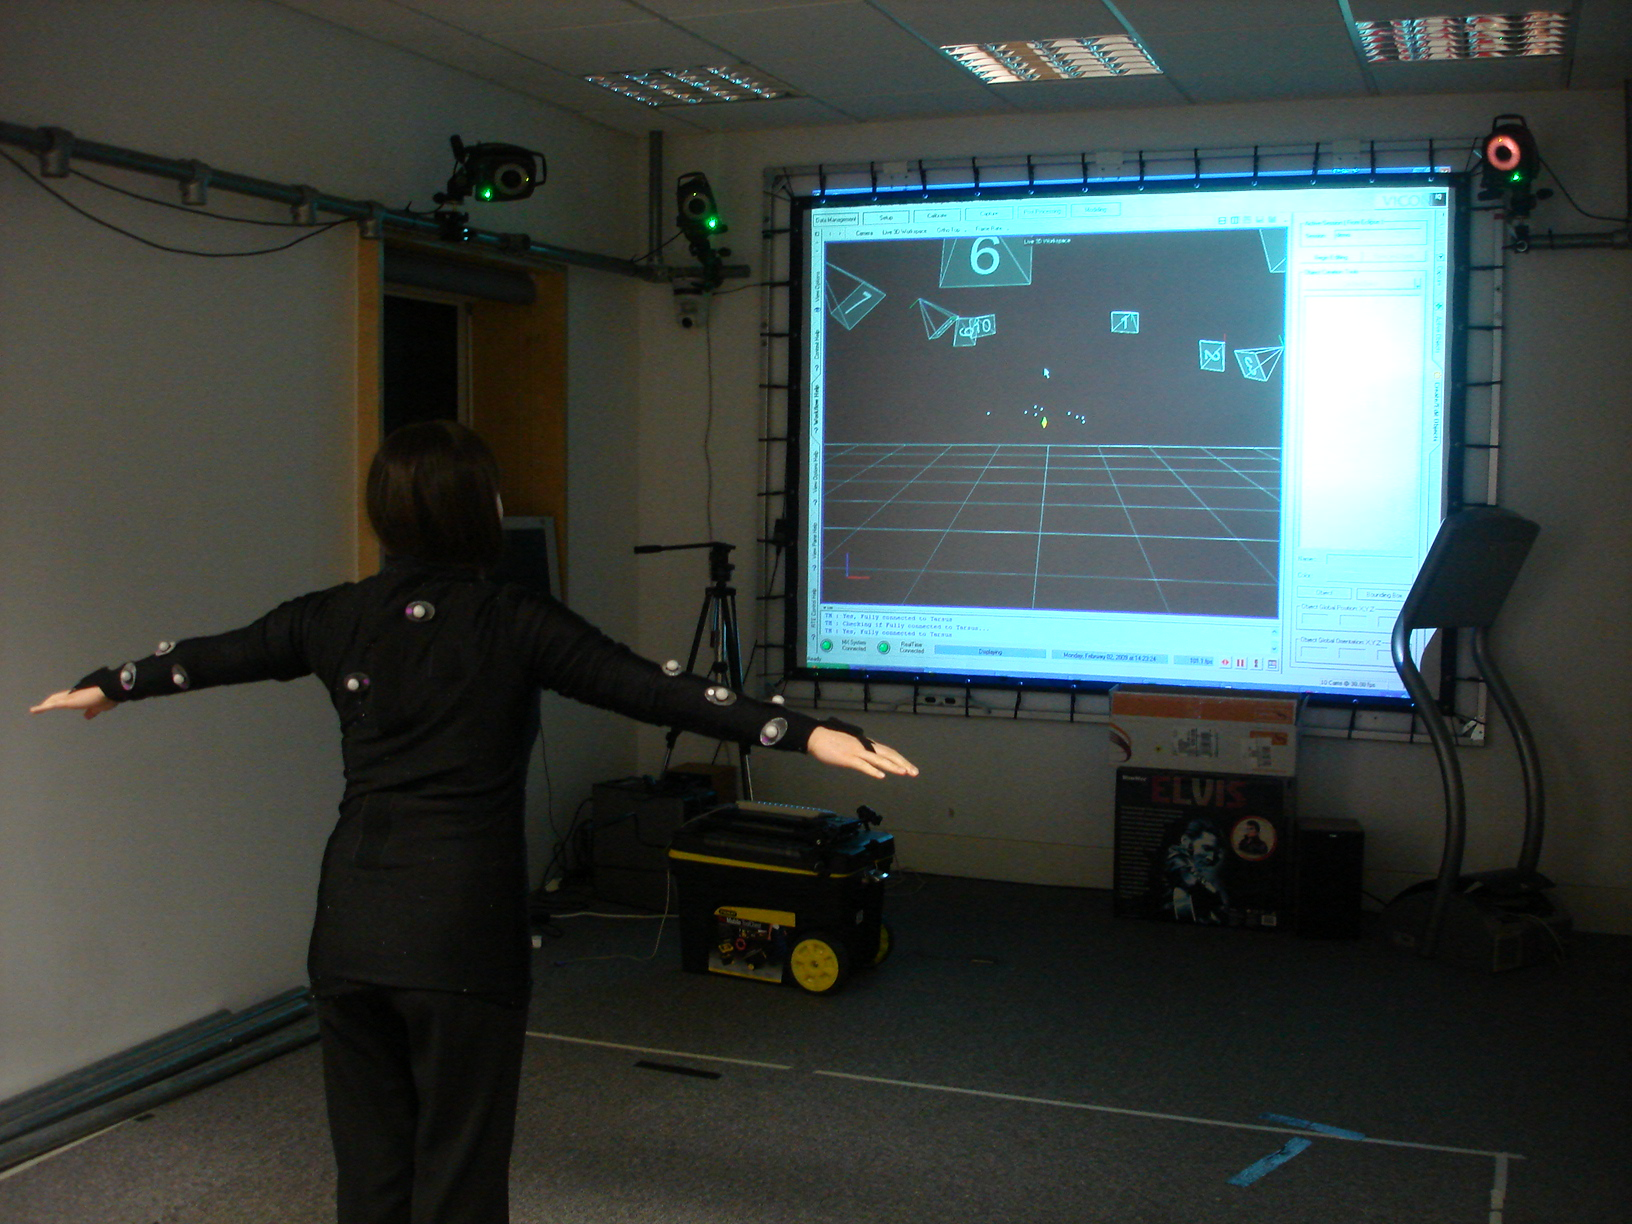
\includegraphics[scale=0.3,angle=0]{images/cherylscreen.ps}
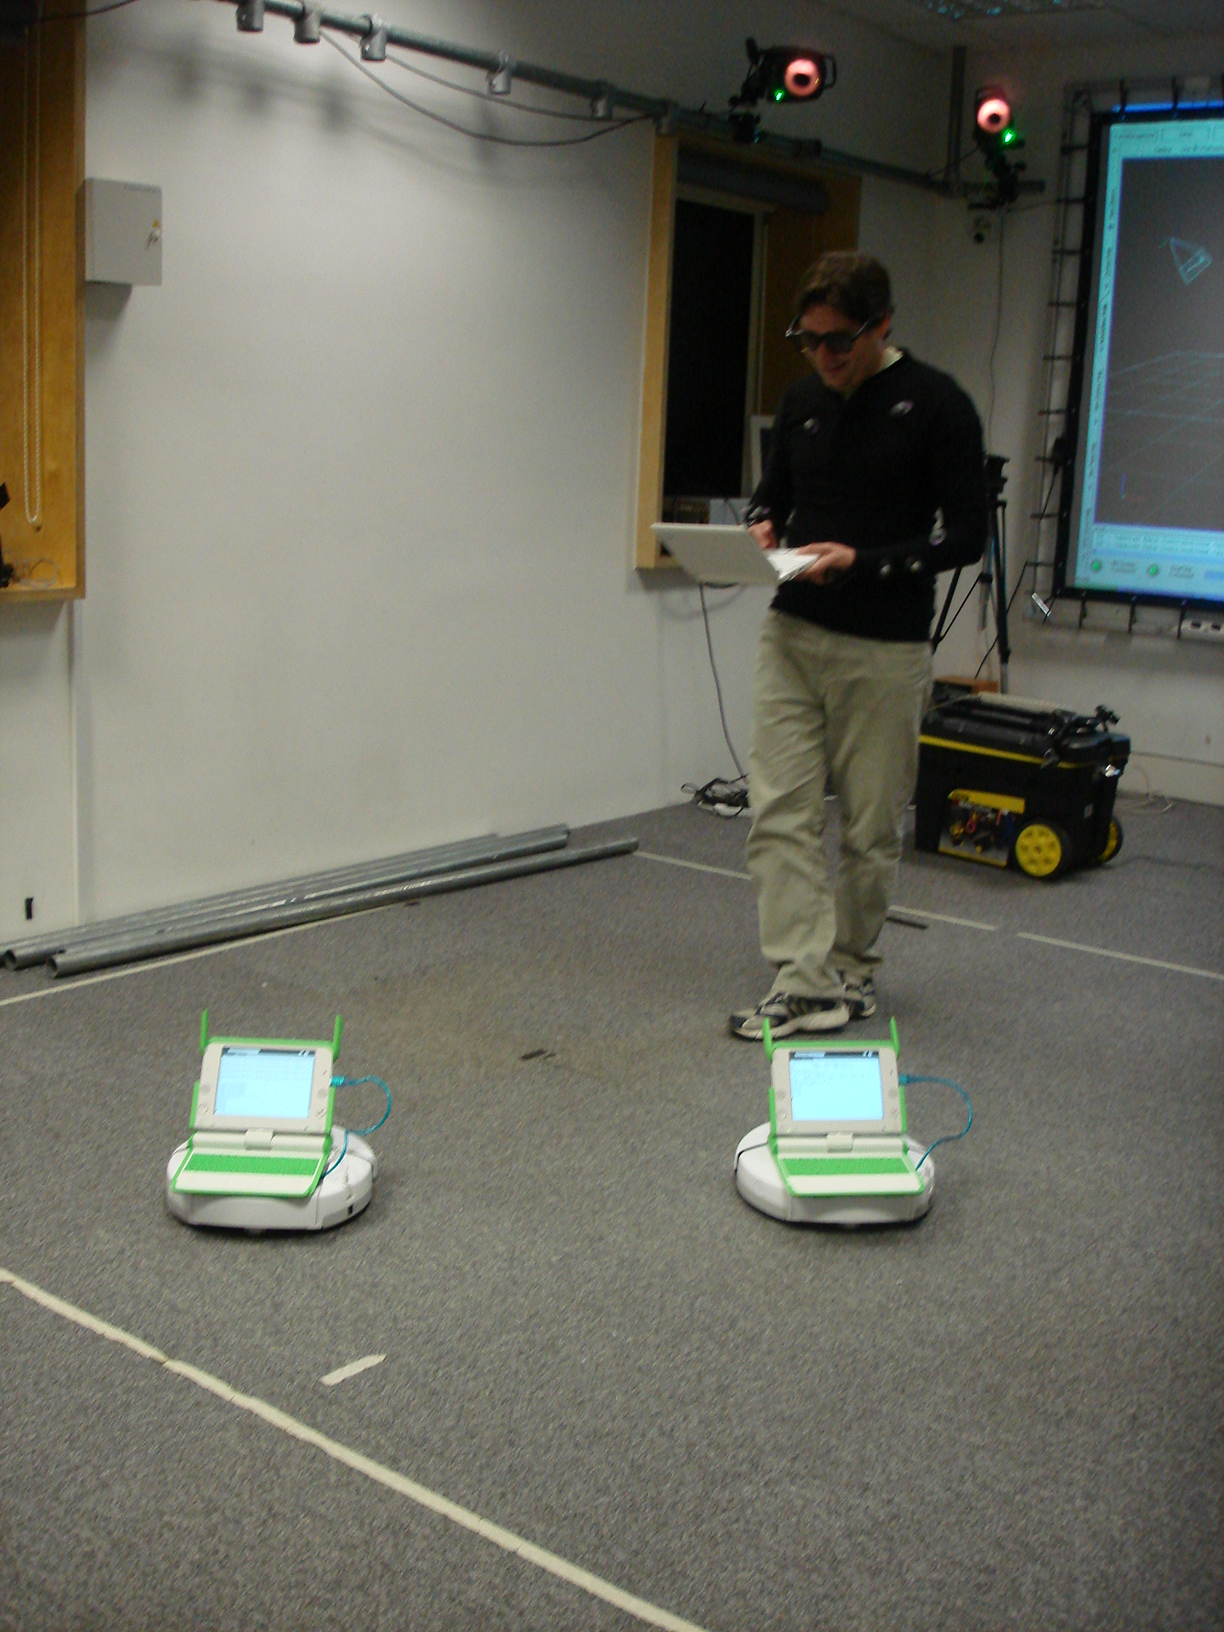
\includegraphics[scale=0.3,angle=0]{images/davidrobots.ps}
\caption{Photographs of demonstrations}
\label{demonstrations}
\end{figure}

Figure \ref{demonstrations} illustrates the alternative methods available for real time control; through arm gestures, or with a mobile device such as a laptop with Control.py running. The robots are connected wirelessly to the WGB network and are set to listen to a single player only, thus demonstrating the multiple user extension. 

Figure \ref{driving} demostrates using the live system; the infra-red cameras are placed around the room, the user wears a black top with twelve markers and the screen projection shows both TARSUS reconstruction and the feedback window, which shows that player 2 is currently not in play.
\begin{figure}
\centering
\includegraphics[scale=0.15,angle=0]{images/live1.ps}
\includegraphics[scale=0.15,angle=0]{images/live2.ps}
\includegraphics[scale=0.15,angle=0]{images/live3.ps}
\includegraphics[scale=0.15,angle=0]{images/live4.ps}
\includegraphics[scale=0.15,angle=0]{images/live5.ps}
\caption{A sequence of stills showing the user issuing an Accelerate and a Turn Right command. The robot responds by moving towards the camera and changing angle.}
\label{driving}
\end{figure}
\section{Successes and failures}

Overall, this project completed its original goals and surpassed them by also implementing extensions. It provides an end-to-end system for conversion of arm gestures into robot control with success rates of over 80\%. In addition to the two originally planned recognisers, I implemented a further two recognisers and a full simulation system for every component of the system.

\chapter{Conclusions}

\section{Achievements}

This project implements a working, complete system which has been demonstrated at the Computer Laboratory Rainbow group Outreach day and tried with multiple users. It combines fundamentally different techniques, and all parts are fully modularised and cleanly separated. This decoupling is a success of software engineering; almost all of the components are testing and can be used as standalone modules.

Integrating five libraries using two languages across three platforms was a major achievement of careful planning and understanding. The plan was completed to a budget, as stated in my project proposal, and the hardware obtained and succesfully integrated into the system. The recognition engine is usable in real-time, offering four classification techniques and 80\% succes rate with two users.

\section{Reflection}

I would like to have experimented with more input devices, as the Vicon system is expensive and time-consuming to set up. For example, accelerometers in the Nintendo Wii and many smartphones would make an ideal handheld controller.

\section{Further work}

Currently, the training and recognition is all performed on a single computer. Since the system is already decoupled, creating a distributed training environment would lead to an improvement in training and recognition times. This would be particularly straightforward given that the Joone library provides support for distributed training, and processing the five hidden Markov models can be done independently.

In the upcoming summer, this system will be used for educational purposes. The extensions which will be implemented in time for the Sutton Trust Summer School include a mobile application for control and writing a multiplayer game using the bump sensors from the robot. I hope that this will encourage others to experiment and interact with the system, testing its robostness and reliability.

\addcontentsline{toc}{chapter}{Bibliography}
\bibliography{dissertation}

\appendix

\chapter{Neural Network recogniser}

\begin{code}
import java.io.*;
import java.util.*;

import org.joone.log.*;
import org.joone.engine.*;
import org.joone.engine.learning.*;
import org.joone.io.*;
import org.joone.net.NeuralNet;

class Neural extends Recogniser implements NeuralNetListener 
{
	static double NEURAL_THRESHOLD = -1;

	static int LEARNING_MODE = -1;
	static int NUM_EPOCHS = -1;
	static int NUM_HIDDEN_NEURONS = -1;
	static double LEARNING_RATE = -1;
	static double MOMENTUM = -1;
	static boolean TRAIN_ON_NEGS = false;
	
	String output_file;
	double err;
	
	LinearLayer input;
	SigmoidLayer hidden, output;
	FullSynapse synapse_IH, synapse_HO;
	NeuralNet nnet;
	Monitor monitor;
	MemoryInputSynapse inputStream, samples;
	TeachingSynapse trainer;
	
	static long timing = System.nanoTime();

	public static Gesture recognise(Person person, Features features)
	{		
		/* Uses:
			features.displacement
			features.leftarm|rightarm.get_delta(0|1|2)
			Total 7 input neurons
		*/
		
		double[] inputdata, outputdata;
		Pattern pin, pout;
		
		init(person); // Check person.nnet has been initialised

		inputdata = new double[Features.num_features];
		features.extract(inputdata);
		pin = new Pattern(inputdata);
		pin.setCount(person.neural_seq++);
		person.nnet.singleStepForward(pin);
		pout = person.netout.fwdGet();
		
		dump_results(pout);
				
		if(NEURAL_THRESHOLD < 0)
			NEURAL_THRESHOLD = Double.valueOf(Config.lookup("neuralthreshold"));
		
		
		double[] a = pout.getArray();
		int command = Gesture.NoMatch;
				
		for (int i = 0; i < Gesture.num_gestures; i++)
		{
			if(a[i] > NEURAL_THRESHOLD)
			{
				if(command == Gesture.NoMatch)
					command = i;
				else
					command = Gesture.MultiMatch;
			}
		}
		
		return new Gesture(command);

	}
		
	void train(ArrayList<Sample> sampleslist, String out_file)
	{

		output_file = out_file;
		Sample samp;
		init_parameters();
		
		int num_samples = sampleslist.size();
		double[][] inputdata = new double[num_samples][Features.num_features];
		double[][] outputdata = new double[num_samples][Gesture.num_gestures];
		for(int i = 0; i < num_samples; i++)
		{
			samp = sampleslist.get(i);
			samp.feat.extract(inputdata[i]);
			for(int j = 0; j < Gesture.num_gestures; j++)
				outputdata[i][j] = 0.0;
			if(samp.gesture.command < Gesture.num_gestures)
				outputdata[i][samp.gesture.command] = 1.0;
		}
		
		input = new LinearLayer();
		hidden = new SigmoidLayer();
		output = new SigmoidLayer();
		input.setLayerName("input");
		hidden.setLayerName("hidden");
		output.setLayerName("output");
		input.setRows(Features.num_features);
		hidden.setRows(NUM_HIDDEN_NEURONS);
		output.setRows(Gesture.num_gestures);
		synapse_IH = new FullSynapse();
		synapse_HO = new FullSynapse();
		synapse_IH.setName("IH");
		synapse_HO.setName("HO");
		input.addOutputSynapse(synapse_IH);
		hidden.addInputSynapse(synapse_IH);
		hidden.addOutputSynapse(synapse_HO);
		output.addInputSynapse(synapse_HO);
		
		inputStream = new MemoryInputSynapse();
		inputStream.setInputArray(inputdata);
		set_columns(inputStream, 1, Features.num_features);
		input.addInputSynapse(inputStream);

		samples = new MemoryInputSynapse();
		samples.setInputArray(outputdata);
		set_columns(samples, 1, Gesture.num_gestures);
			
		trainer = new TeachingSynapse();
		trainer.setDesired(samples);
		output.addOutputSynapse(trainer);
			
		nnet = new NeuralNet();
		nnet.addLayer(input, NeuralNet.INPUT_LAYER);
		nnet.addLayer(hidden, NeuralNet.HIDDEN_LAYER);
		nnet.addLayer(output, NeuralNet.OUTPUT_LAYER);
		
		monitor = nnet.getMonitor();
		monitor.setTrainingPatterns(num_samples);
		monitor.setTotCicles(NUM_EPOCHS);
		monitor.setLearningRate(LEARNING_RATE);
		monitor.setMomentum(MOMENTUM);
		monitor.setLearning(true);
		
		//Add learner
		
		monitor.addLearner(0, "org.joone.engine.BasicLearner"); // On-line
		monitor.addLearner(1, "org.joone.engine.BatchLearner"); // Batch
		monitor.addLearner(2, "org.joone.engine.RpropLearner"); // RPROP
		
		monitor.setLearningMode(LEARNING_MODE);
				
		monitor.setSingleThreadMode(true);
		monitor.addNeuralNetListener(this);
			
		nnet.go();
	}
	
	private void init_parameters()
	{
		if(LEARNING_MODE < 0)
			LEARNING_MODE = Integer.valueOf(Config.lookup("n_learner"));
		if(NUM_EPOCHS < 0)
			NUM_EPOCHS = Integer.valueOf(Config.lookup("n_epochs"));
		if(NUM_HIDDEN_NEURONS < 0)
			NUM_HIDDEN_NEURONS = Integer.valueOf(Config.lookup("n_hidden_nodes"));
		if(LEARNING_RATE < 0)
			LEARNING_RATE = Double.valueOf(Config.lookup("n_learning_rate"));
		if(MOMENTUM < 0)
			MOMENTUM = Double.valueOf(Config.lookup("n_momentum"));
		if(TRAIN_ON_NEGS == false)
			TRAIN_ON_NEGS = Boolean.valueOf(Config.lookup("n_train_on_negs"));
		
		if (LEARNING_MODE == 2)
		{
			LEARNING_RATE = 1.0;
		}
	}
	
	private void set_columns(MemoryInputSynapse syn, int first, int last)
	{
		String cols = "";
		
		for(int i = first; i <= last; i++)
		{
			if(i == last)
				cols = cols + i;
			else
				cols = cols + i + ",";
		}
		syn.setAdvancedColumnSelector(cols);
	}
		
	// NeuralNetListener interface methods follow:
	
	public void errorChanged(NeuralNetEvent e)
	{
		int cycle;
		
		Monitor mon = (Monitor)e.getSource();
		cycle = mon.getCurrentCicle();
		if(cycle % (NUM_EPOCHS/10) == 0 || cycle >= NUM_EPOCHS - 10)
		{
			err = mon.getGlobalError();
			Utils.log(String.format("%d", cycle) + " epochs remaining; RMSE = " 
			    + String.format("%5f", err));
	    }
	}
	
	public void netStarted(NeuralNetEvent e)
	{
		Utils.log("Training started");
		timing = System.nanoTime();
	}
	
	public void netStopped(NeuralNetEvent e)
	{
		timing = System.nanoTime() - timing;
		Utils.log("Learning-mode Learning-rate Momentum Epochs Hidden-nodes ns RMSE");
		Utils.results(LEARNING_MODE + " " + LEARNING_RATE + " " + MOMENTUM + " " + NUM_EPOCHS + " " + NUM_HIDDEN_NEURONS + " " + timing + " " + String.format("%5f", err));
		saveNeuralNet(nnet, output_file);
	}
	
	public void netStoppedError(NeuralNetEvent e, String error)
	{
		Utils.log("Net stopped error: " + error);
	}
	
	public void cicleTerminated(NeuralNetEvent e) {}
	
	static void saveNeuralNet(NeuralNet nnet, String filename)	
	{
		try
		{
			FileOutputStream stream = new FileOutputStream(filename);
			ObjectOutputStream out = new ObjectOutputStream(stream);
			out.writeObject(nnet);
			out.close();
		}
		catch(Exception e)
		{
			Utils.error("Cannot save neural net to <" + filename + ">");
		}
	}
		
	static NeuralNet restoreNeuralNet(String filename)
	{
		try
		{
			FileInputStream stream = new FileInputStream(filename);
			ObjectInputStream in = new ObjectInputStream(stream);
			return (NeuralNet)in.readObject();
		}
		catch(Exception e)
		{
			Utils.error("Cannot load neural net from <" + filename + ">");
		}
		return null; // Never happens
	}
	
	static void dump_results(Pattern pat)
	{
		double[] a = pat.getArray();
		Gesture gest = new Gesture(0);
		
		assert(a.length == Gesture.num_gestures);
		for(int i = 0; i < Gesture.num_gestures; i++)
		{
			gest.command = i;
			if (Utils.verbose)
				System.out.printf(gest.toString() + ": %5f\n", a[i]);
		}
	}
	
	static void init(Person p)
	{
		Layer input, output;

		if(p.nnet != null)
			return; // Already initialised
			
		p.nnet = restoreNeuralNet(p.neural_file);
		
		input = p.nnet.getInputLayer();
		input.removeAllInputs();
		
		output = p.nnet.getOutputLayer();
		output.removeAllOutputs();
		
		p.netout = new DirectSynapse();
		output.addOutputSynapse(p.netout);
		
		p.nnet.getMonitor().setLearning(false);
	}
}
\end{code}

\chapter{Hidden Markov model recogniser}
\begin{code}
import java.io.*;
import java.util.*;

import java.util.ArrayList;
import java.util.List;

import be.ac.ulg.montefiore.run.jahmm.*;
import be.ac.ulg.montefiore.run.jahmm.learn.*;
import be.ac.ulg.montefiore.run.jahmm.io.*;

class Markov extends Recogniser
{

	ArrayList<Learner> learners;
	ArrayList<ArrayList<ArrayList<ObservationVector>>> sequences;
	
	static final int NUM_DIMENSIONS = 9;
	static int NUM_STATES = -1;
	static int NUM_ITERATIONS = -1;
	static int LEARNER = -1;
	
	String output_root;
	
	static int SCALING_FACTOR = 100;
	
	public static Gesture recognise(Person person, Features features)
	{
		String filename;
		double[] probabilities = new double[Gesture.num_gestures];
		ArrayList<ObservationVector> framedata = toObservationVectors(features.rawdata);
		
		Hmm<ObservationVector> recog_hmm = new Hmm<ObservationVector>(5, new OpdfMultiGaussianFactory(features.rawdata.size()));
				
		for (int i = 0; i < Gesture.num_gestures; i++)
		{
			filename  = person.markov_root + new Gesture(i).toAction();
			recog_hmm = restore_hmm(filename);
			probabilities[i] = recog_hmm.lnProbability(framedata);
		}

		dump_results(probabilities);

		int command = Gesture.NoMatch;
				
		for (int i = 0; i < Gesture.num_gestures; i++)
		{
			if(!Double.isNaN(probabilities[i]))
			{
				if(command == Gesture.NoMatch)
					command = i;
				else
					command = Gesture.MultiMatch;
			}
		}

		return new Gesture(command);
	}

	static void dump_results(double[] a)
	{
		Gesture gest = new Gesture(0);
		
		assert(a.length == Gesture.num_gestures);
		for(int i = 0; i < Gesture.num_gestures; i++)
		{
			gest.command = i;
			Utils.log(gest.toString() + ": " + String.format("%5f", a[i]));
		}
	}

	void train(ArrayList<Sample> samples, String out_file)
	{
		init_parameters();
		output_root = out_file;

		for (Sample sample : samples)
		{
			Learner learner = learners.get(sample.gesture.command);
			learner.add_sequence(toObservationVectors(sample.data));
			Utils.log("Assigned " + sample.pathname +
			 " to learner for " + learner.gesture.toString());
		}
		
		long timing = System.nanoTime();
		
		for (Learner learner : learners)
		{
			Utils.log("Training " + learner.gesture.toString());
			if (LEARNER == 0)
			{	
				learner.learnbw();
			}
			else if (LEARNER == 1)
			{
				learner.learnkm();
			}
			else
			{
				Utils.error("Unknown learner; valid options are " +
					"0 for Baulm-Welch and 1 for K-Means");
			}
			
			save_hmm(learner, output_root + "_" + learner.gesture.toAction());
		}
		
        timing = System.nanoTime() - timing;
        
        Utils.log("Learner hidden-states iterations ms");
        Utils.results(LEARNER + " " + NUM_STATES + " " + NUM_ITERATIONS + " " + timing/1000);
	}

	private static ArrayList<ObservationVector> toObservationVectors(ArrayList<Frame> frames)
	{
		ArrayList<ObservationVector> ovs = new ArrayList<ObservationVector>();
		double[] values;
		
		for (int i = 0; i < frames.size(); i++)
		{
			values = frames.get(i).toDoubles();
			for (double v : values)
			{
				v  = v / SCALING_FACTOR;
			}
			ovs.add(new ObservationVector(values));
		}
		//System.out.println("Done sample " + s.pathname);
		return ovs;
	}
		
	static void save_hmm(Learner learner, String filename)
	{
		try
		{
			FileOutputStream stream = new FileOutputStream(filename);
			ObjectOutputStream out = new ObjectOutputStream(stream);
			out.writeObject(learner.hmm);
			out.close();
		    Utils.log("Hmm saved to " + filename);
		}
		catch (IOException e)
		{
			Utils.error("Cannot save hidden markov model to <" + filename + ">");
		}
	}
	
	static Hmm restore_hmm(String filename)
	{
		try
		{
			FileInputStream stream = new FileInputStream(filename);
			ObjectInputStream in = new ObjectInputStream(stream);
		    Utils.log("Hmm loaded from " + filename);
			return (Hmm)in.readObject();
		}
		catch (IOException e)
		{
			Utils.error("Cannot load hidden markov model from <" + filename + ">");
		}
		catch (Exception e)
		{}
		return null;
	}

	private void init_parameters()
	{
		if(NUM_STATES < 0)
			NUM_STATES = Integer.valueOf(Config.lookup("m_hidden_states"));
		if(NUM_ITERATIONS < 0)
			NUM_ITERATIONS = Integer.valueOf(Config.lookup("m_iterations"));
		if(LEARNER < 0)
			LEARNER = Integer.valueOf(Config.lookup("m_learner"));

		learners = new ArrayList<Learner>(5);

		for (int i = 0; i < Gesture.num_gestures; i++)
		{
			learners.add(new Learner(NUM_STATES, NUM_DIMENSIONS, NUM_ITERATIONS,
				new Gesture(i)));
		}
	}
};

class Learner
{
	Hmm<ObservationVector> hmm;
	ArrayList<ArrayList<ObservationVector>> sequences;
	BaumWelchScaledLearner bwl;
	KMeansLearner<ObservationVector> kml; 
    OpdfMultiGaussianFactory factory;
    Gesture gesture;
    
	int num_states;
	int num_dimensions;
	int num_iterations;    

	Learner(int states, int dimensions, int iterations, Gesture g)
	{
		num_states = states;
		num_dimensions = dimensions;
		num_iterations = iterations;
		gesture = g;

		factory = new OpdfMultiGaussianFactory(num_dimensions);
		hmm = new Hmm<ObservationVector>(num_states, factory);
		sequences = new ArrayList<ArrayList<ObservationVector>>();
	}
	
	void add_sequence(ArrayList<ObservationVector> seq)
	{
		sequences.add(seq);
	}
	
	void learnbw()
	{
		bwl = new BaumWelchScaledLearner();
		bwl.setNbIterations(num_iterations);
		//One iteration of KMeansLearner to initalise
		hmm = new KMeansLearner<ObservationVector>(num_states, factory, sequences).iterate();
		hmm = bwl.learn(hmm, sequences);
	}
	
	void learnkm()
	{
		kml = new KMeansLearner<ObservationVector>(num_states, factory, sequences);
		hmm = kml.learn();
	}
}
\end{code}

\chapter{Control.py}

\begin{code}
from Tkinter import *
import scop

class Controls(Frame):
    """This class provides mousebutton and arrow key support for emitting basic controls (a,d,l,r,s) to an SCOP socket."""

    def __init__(self, parent, sock, player, width=800, height=800, **options):
        Frame.__init__(self, parent, **options)
        self.width, self.height = width, height
        parent.title("Player " + str(player))
        self.sock = sock     
        
        Button(self, text='accel', command=self.Accelerate).grid(row=0, column=1)
        Button(self, text='decel', command=self.Decelerate).grid(row=2, column=1)
        Button(self, text='left', command=self.TurnLeft).grid(row=1, column=0)
        Button(self, text='right', command=self.TurnRight).grid(row=1, column=2)
        Button(self, text='startstop', command=self.Pause).grid(row=1, column=1)

        self.running = 0
        self.period = 20 # milliseconds

        parent.bind('<KeyPress-Left>', self.TurnLeft)
        parent.bind('<KeyPress-Right>', self.TurnRight)
        parent.bind('<KeyPress-Up>', self.Accelerate)
        parent.bind('<KeyPress-Down>', self.Decelerate)
        parent.bind('<KeyPress-space>', self.Pause)

    def Accelerate(self, event=None):
        scop.scop_emit(self.sock, "a")

    def Decelerate(self, event=None):
        scop.scop_emit(self.sock, "d")

    def TurnLeft(self, event=None):
        scop.scop_emit(self.sock, "l")

    def TurnRight(self, event=None):
        scop.scop_emit(self.sock, "r")
        
    def Pause(self, event=None):
	if self.running:
	    self.running = 0
	    scop.scop_emit(self.sock, "s")
	else:
	    self.running = 1
	    scop.scop_emit(self.sock, "s")
\end{code}

\cleardoublepage

\chapter{Project Proposal}


% Draft #1 (final?)

\vfil

\centerline{\Large Diploma in Computer Science Project Proposal}
\vspace{0.4in}
\centerline{\Large How to write a dissertation in \LaTeX\ }
\vspace{0.4in}
\centerline{\large M. Richards, St John's College}
\vspace{0.3in}
\centerline{\large Originator: Dr M. Richards}
\vspace{0.3in}
\centerline{\large 21 November 2000}

\vfil

\subsection*{Special Resources Required}
File space on Thor -- 25Mbytes\\
Account on the DEC Workstations -- 15Mbytes\\
An account on Ouse\\
The use of my own IBM PC (1000GHz Pentium, 200Mb RAM and 40Gb Disk).
\vspace{0.2in}

\noindent
{\bf Project Supervisor:} Dr M. Richards
\vspace{0.2in}

\noindent
{\bf Director of Studies:} Dr M. Richards
\vspace{0.2in}
\noindent
 
\noindent
{\bf Project Overseers:} Dr~F.~H.~King  \& Dr~S.~W.~Moore

\vfil
\pagebreak

% Main document

\section*{Introduction}

Many students write their CST and Diploma dissertations in \LaTeX\ and
spend a fair amount of time learning just how to do that. The purpos of 
this project is to write a demonsatration dissertation that explains in
detail how it done and how the result can be given to the Bookshop
on an MSDOS floppy disk for printing and binding.

\section*{Work that has to be done}

The project breaks down into the following main sections:-

\begin{enumerate}

\item The construction of a skeleton dissertation with the required 
structure. This involves writing the Makefile and makeing dummy files
for the title page, the proforma, chapters 1 to 5, the appendices and
the proposal.

\item Filling in the details required in the cover page and proforma.

\item Writing the contents of chapters 1 to 5, including examples
of common \LaTeX\ constructs.

\item Adding a example of how to use floating figures and encapsulated
postscript diagrams.

\end{enumerate}

\section*{Difficulties to Overcome}

The following main learning tasks will have to be undertaken before 
the project can be started:

\begin{itemize}

\item To learn \LaTeX\ and its use on Thor.

\item To discover how to incorporate encapsulated postscript into
a \LaTeX\ document, and to find a suitable drawing package on Thor
to recommend.

\item To discover what format the Bookshop would like for the finished
dissertation, and how to deal with postscript files that are too
large to fit on a single floppy disk.

\end{itemize}



\section*{Starting Point}

I have a reasonable working knowledge of \LaTeX\ and have convenient
access to Thor using an IBM PC in my office. Writing MSDOS disks is no 
problem.

\section*{Resources}

This project requires little file space so 25Mbytes of disk space on Thor
should be sufficient. I plan to use my own IBM PC to write floppy disks, 
but could use the PWF PCs if my own machine breaks down. 

Backup will be on floppy disks.

\section*{Work Plan}

Planned starting date is 01/12/2000.

\subsection*{Michaelmas Term} 

By the end of this term I intend to have completed the learning tasks 
outlined in the relevant section.


\subsection*{Lent Term}

By the division of term the overall structure of the dissertation
will have been written and tested.

By the end of term, example figures using encapsulated postscript
will have been included.
 

\subsection*{Easter Term}

On completion of the exams I will incorporate final details into 
the dissertation including a bibliography using bibtex and a table of contents.
The estimated completion date being 25/07/2001 to allow 
plenty of time should any unforeseen problems arise.



%\input{...}

\end{document}
